\chapter{\uppercase{Implementation Results}}\label{TPSframeworkResults} % of the Framework

This chapter presents the results obtained through the application of the proposed \emph{training point selection and error estimation framework}. The discussions can be grouped as listed below:
\begin{itemize}  
\item Validating the proposed error estimates for surrogate models (\emph{root mean square discrepancy} and \emph{maximum absolute discrepancy}) by comparing them with the actual error measures of the surrogate model 
(\emph{root mean square error} and \emph{maximum absolute error}),
\item Demonstrating the superiority of the proposed ``dynamic'' training point selection versus other popular training point selection approaches such as LHS, low-discrepancy sequences and kriging MSE minimization in terms of \emph{model accuracy} and \emph{monotonicity}. Another motive is addressing the question of training point selection under the availability of gradient and Hessian information,
\item Establishing the ``non-intrusiveness'' of the proposed framework by effective integration with two different surrogate models: the kriging and polynomial chaos expansions (PCE),
\item Discussing results pertaining to Hessian-enhanced polynomial chaos which is one of the new contributions of this work,
\item Presenting guidelines to users for a better combination of training point selection with higher-order derivative information, benchmarked based on \emph{equivalent computational time} and their corresponding \emph{accuracy},
%\item demonstrating the advantage of variable-fidelity information in surrogate building in terms of \emph{computational time} and \emph{accuracy},
\item Comparing the performance of kriging and polynomial chaos with each other  in terms of \emph{accuracy}, \emph{robustness}, and \emph{computational time}.
\end{itemize}
Data and results for the aforementioned discussions are shown for multi-dimensional analytical test functions which are defined next.


\section{Analytical Test functions}
\label{testcases}

Eqns.~\eqref{f1},~\eqref{f2} and~\eqref{f3} list the multidimensional exponential, Runge, and Rosenbrock test functions, respectively, which are used for evaluation purposes on an $M$-dimensional hypercube \mbox{$[-2,2]^M$}.
\begin{gather}
%\item A multi-dimensional Cosine function: $f_1(x_1,\ldots,x_M)=\cos(x_1 + \ldots + x_M)$
f_1(x_1,\ldots,x_M)=\mathrm{e}^{(x_1 + \ldots + x_M)}\label{f1}\\
f_2(x_1,\ldots,x_M)=\frac{1}{1+x_1^2 + \ldots + x_M^2}\label{f2}\\
f_3(x_1,\ldots,x_M)=\sum_{i=1}^{M-1} \left[ (1-x_i)^2+100(x_{i+1}-x_i^2)^2\right]\label{f3}
\end{gather}
The choice of these three analytical test functions is due to the
reasons outlined below. The first test function $f_1$ features an
infinite Taylor's series expansion and it can not be captured ``exactly''
by any polynomial. The Runge function $f_2$ being a rational polynomial is known to pose difficulties for polynomial based response surfaces~\cite{Constantine2013}. The Rosenbrock function is a popular test problem for gradient based optimizations, and being a fourth order polynomial it is captured exactly by any polynomial of order greater than or equal to four. A two-dimensional surface contour plot for each of the above test functions is shown in Figure~\ref{fig:3d_contour_test_functions}.
\begin{figure}[h]
\centering
\begin{minipage}[b]{0.32\linewidth}
  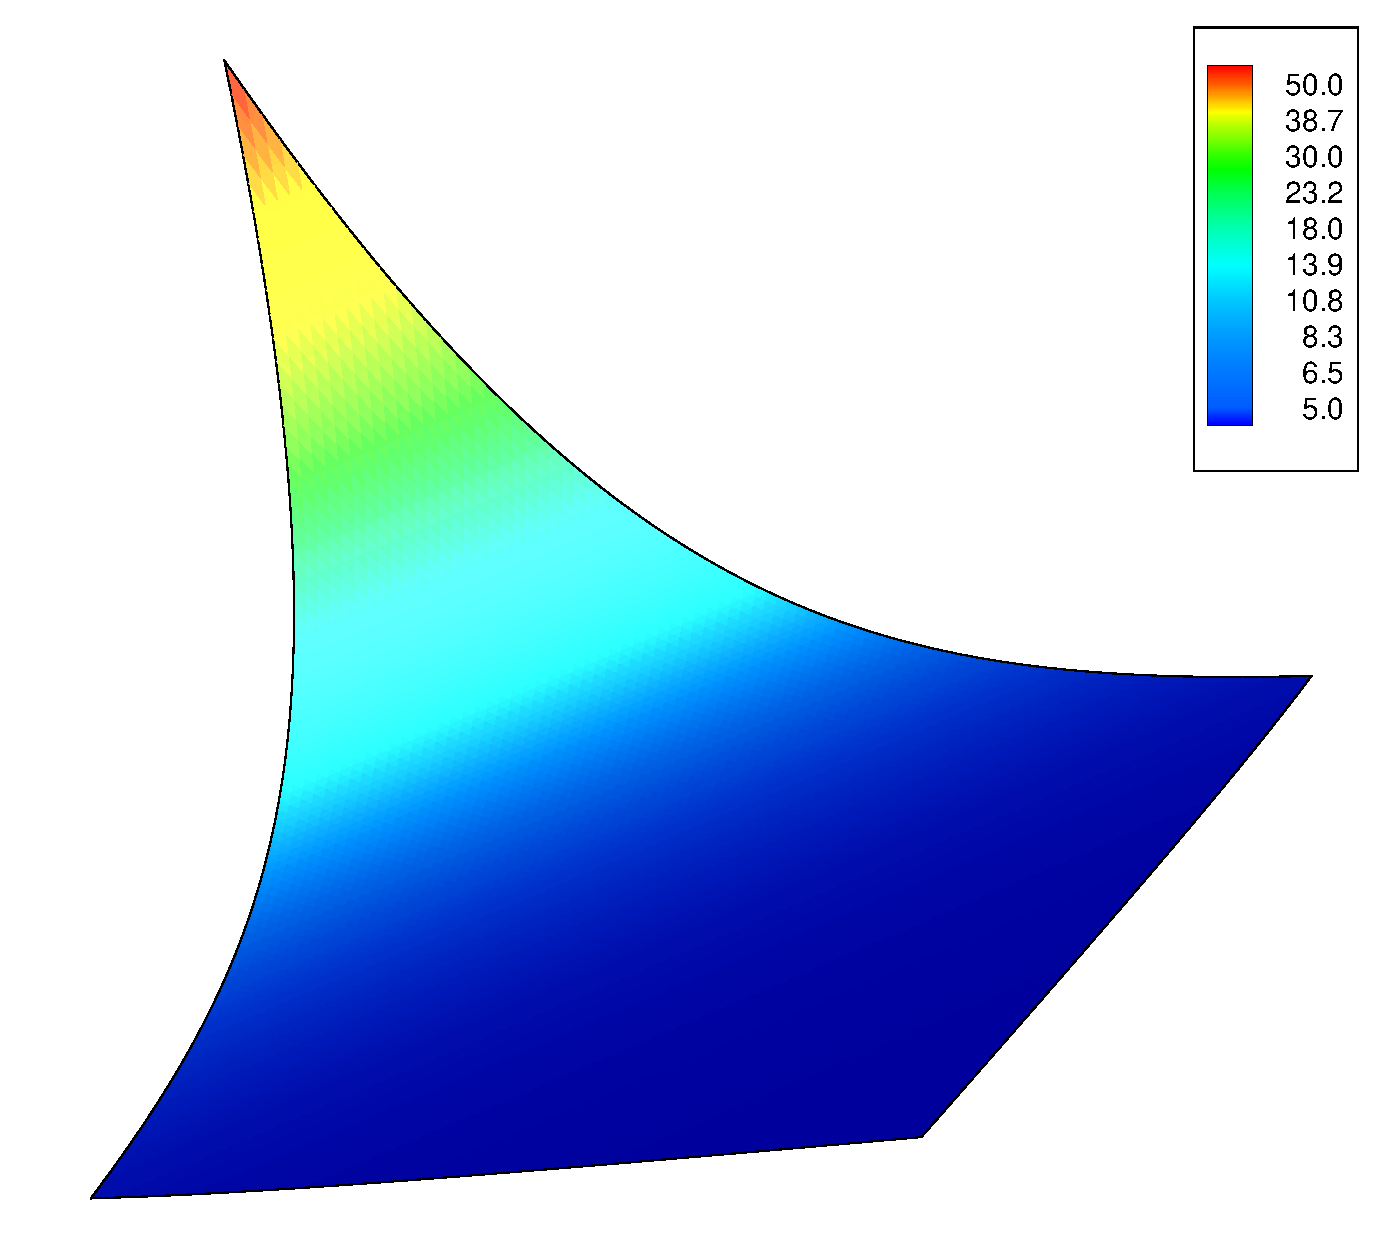
\includegraphics[width=1.0\textwidth]{exp3d.eps} \subcaption{Exponential}
\end{minipage}
\begin{minipage}[b]{0.32\linewidth}
  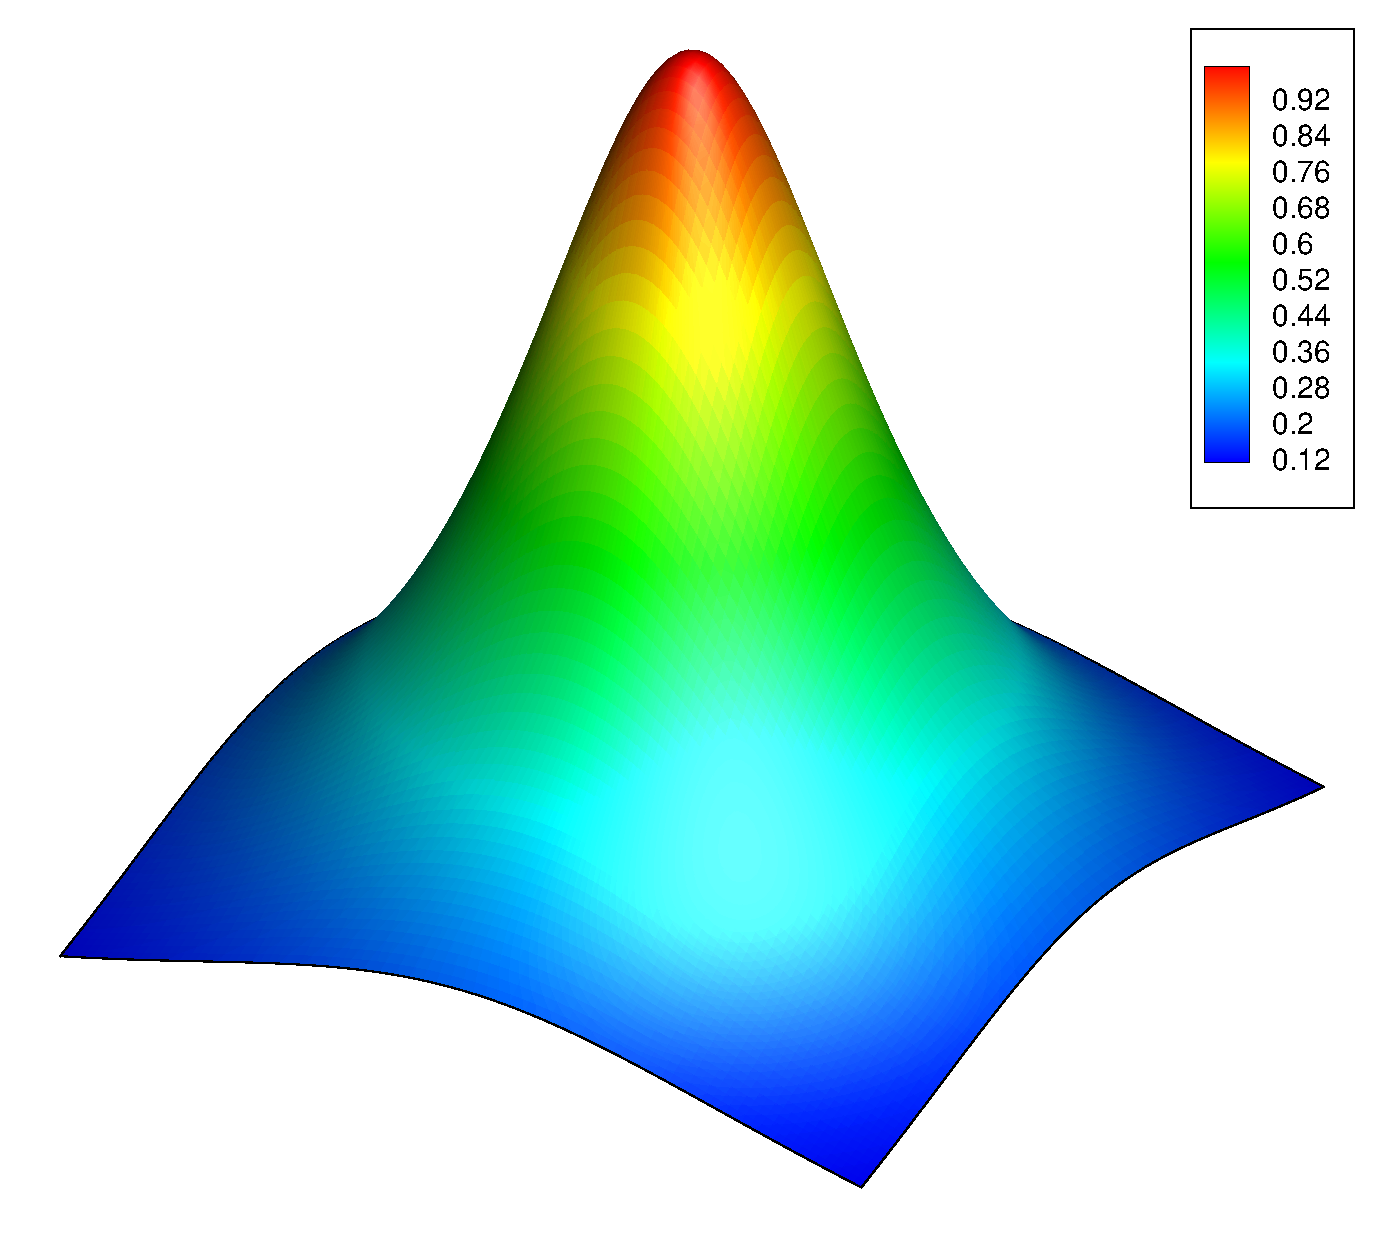
\includegraphics[width=1.0\textwidth]{runge3d.eps} \subcaption{Runge}
\end{minipage}
\begin{minipage}[b]{0.32\linewidth}
 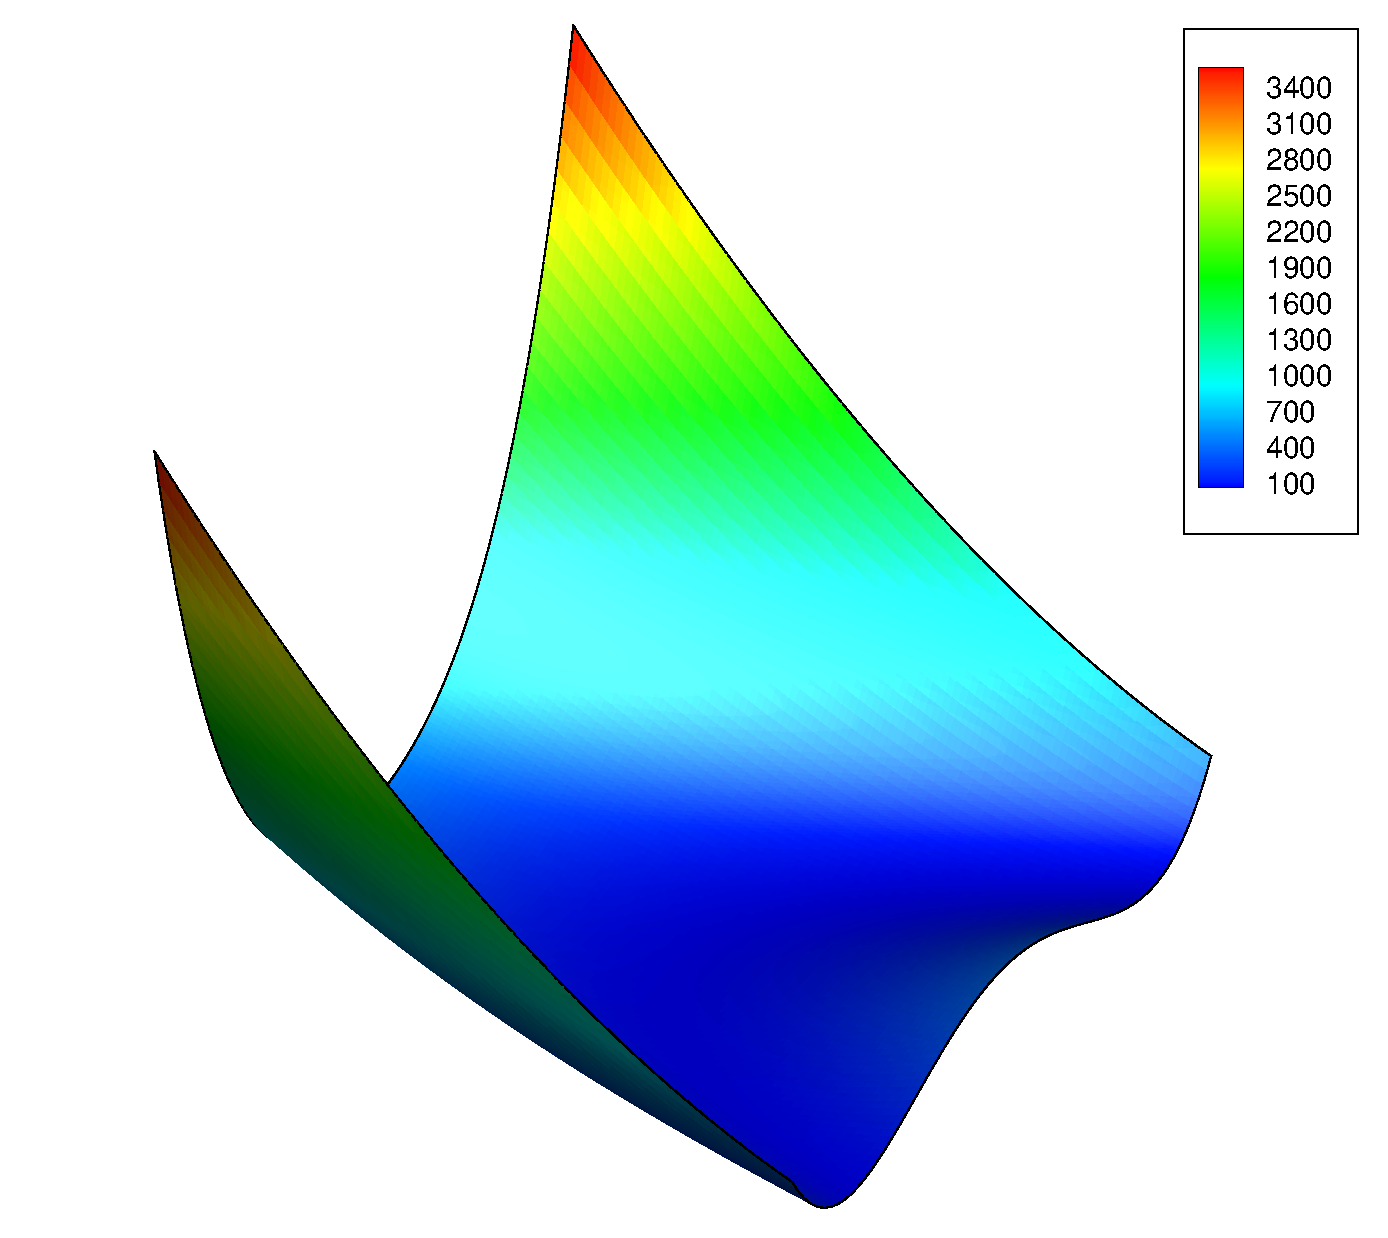
\includegraphics[width=1.0\textwidth]{rosen3d.eps} \subcaption{Rosenbrock}
\end{minipage}
\caption[Contours of analytical test function.]{Contour plots of analytical test functions in two dimensions where the contours are colored by the function values.}
\label{fig:3d_contour_test_functions}
\end{figure} 
\\\\
The root mean square error (RMSE) between the exact $f(\x)$ and approximated function values $\widehat{f}(\x)$ is calculated on an $M$-dimensional Cartesian mesh with $N_t$ total nodes. Mathematically,
\beq
\textrm{RMSE}={\sqrt{\frac{1}{N_t}{\sum_{i=1}^{N_t}}(f^{(i)}-\widehat{f}^{(i)})^2}}.
\label{RMSE}
\eeq
The RMSE is calculated on a Cartesian mesh with $10,201$ and $100,000$ nodes for two- and five-dimensional test cases, respectively.



\section{Validation of Proposed Error Estimates}\label{rmsddemo}

%Conventional methods such as cross validation~\cite{CVOriginal,CrossValidation1}  are being used for validating the surrogate model.
As discussed in section~\ref{dynamic}, the dynamic training point
selection framework also provides an error estimate for the global (main) surrogate model through the maximum absolute discrepancy (MAD) and the root mean square discrepancy (RMSD).


\subsection{Comparison with Actual Errors and Cross Validation}

In this section, comparisons of: $(i)$ the actual maximum absolute error (MAE or $L_\infty$-norm) and the maximum cross validation error (Max--CVE) with the proposed MAD, and $(ii)$  the actual root mean square error (RMSE or $L_2$-norm) and mean cross validation error (MCVE) with the proposed RMSD, are provided. Figures~\ref{diffrmsekrig} and~\ref{diffrmsePCE} show the above mentioned comparisons for kriging and PCE, respectively. A \emph{leave-one-out cross validation}~\cite{CVOriginal,CrossValidation1} is employed in this study.

\begin{figure}[h]
  \centering
\begin{minipage}[b]{0.32\linewidth}
  \includegraphics[width=1.0\textwidth]{exponential1KR.eps} \subcaption{Exponential} %\caption{Cosine}
\end{minipage}
\begin{minipage}[b]{0.32\linewidth}
  \includegraphics[width=1.0\textwidth]{runge10KR.eps}\subcaption{Runge} %\caption{Runge}
\end{minipage}
\begin{minipage}[b]{0.32\linewidth}
  \includegraphics[width=1.0\textwidth]{rosenKR.eps} \subcaption{Rosenbrock} %\caption{Exponential}
\end{minipage}
\caption[Proposed error measures versus  actual errors and CV using kriging.]{A comparison of  the proposed error measures (blue lines) with actual errors (red lines) and leave-one-out cross validation (green lines) on two-dimensional test functions using kriging.}
\label{diffrmsekrig}
\end{figure}
\begin{figure}[h]
  \centering
\begin{minipage}[b]{0.32\linewidth}
  \includegraphics[width=1.0\textwidth]{exponential1PC.eps} \subcaption{Exponential}%\caption{Cosine}
\end{minipage}
\begin{minipage}[b]{0.32\linewidth}
  \includegraphics[width=1.0\textwidth]{runge10PC.eps} \subcaption{Runge} %\caption{Runge} 
\end{minipage}
\begin{minipage}[b]{0.32\linewidth}
  \includegraphics[width=1.0\textwidth]{rosenPC.eps} \subcaption{Rosenbrock} %\caption{Exponential}
\end{minipage}
\caption[Proposed error measures versus  actual errors and CV using PCE.]{A comparison of the  proposed error measures (blue lines) with actual errors (red lines) and leave-one-out cross validation (green lines) on two-dimensional test functions using PCE.}
\label{diffrmsePCE}
\end{figure}


The general observation is that both the proposed error measures (MAD and RMSD) feature an excellent agreement with the actual errors (MAE and RMSE) for all tested cases (exponential, Runge and Rosenbrock functions) 
and surrogate modeling approaches (kriging and PCE), with only a few occasional minor differences.
This presented behavior shows great promise to validate the surrogate model without warranting exact function evaluations in applications of practical interest.
Cross validation exhibits satisfactory tendencies in matching the actual errors but its overall performance is more chaotic.
For all test cases a maximum of twenty-five nearest existing training points are used to build local approximations with MIR. 


\subsection{Comparison with Error Distributions in the Domain}


In Figures~\ref{diffrmsekrig} and~\ref{diffrmsePCE} quantitative metrics have been used to validate the proposed error estimate for surrogate models. 
This section is intended to provide an insight into the spatial distribution of  the \emph{actual error, $\epsilon$,} and the \emph{proposed discrepancy, $\delta$}. Figures~\ref{Expdist},~\ref{Rungedist} and~\ref{Rosendist} show contour plots of the distribution of: $(i)$ the local surrogate model error, $\epsilon_{local}=|f-\widehat{f}_{local}|$, $(ii)$ the global kriging surrogate model error, $\epsilon_{global}=|f-\widehat{f}_{global}|$, and $(iii)$ the proposed discrepancy function, $\delta=|\widehat{f}_{local}-\widehat{f}_{global}|$, for the exponential, Runge and Rosenbrock test functions, respectively.



 The main assumption of the framework has been that the local surrogate models provide a more accurate representation of their corresponding sub-domain than the global surrogate model. The local and global surrogate model errors shown in the leftmost and middle contour plots of Figures~\ref{Expdist},~\ref{Rungedist} and \ref{Rosendist} reveal that the local surrogate models are more accurate than the global surrogate model.
For all the cases the local surrogate models use the closest 25 data points to predict the function value at a test location.
For the Rosenbrock test function (see Figure~\ref{Rosendist}) the local surrogate is indeed a ``second global surrogate model'' as all the available data (25 points) is used for its predictions. 


\begin{figure}[h]
  \centering
\begin{minipage}[b]{0.32\linewidth}
  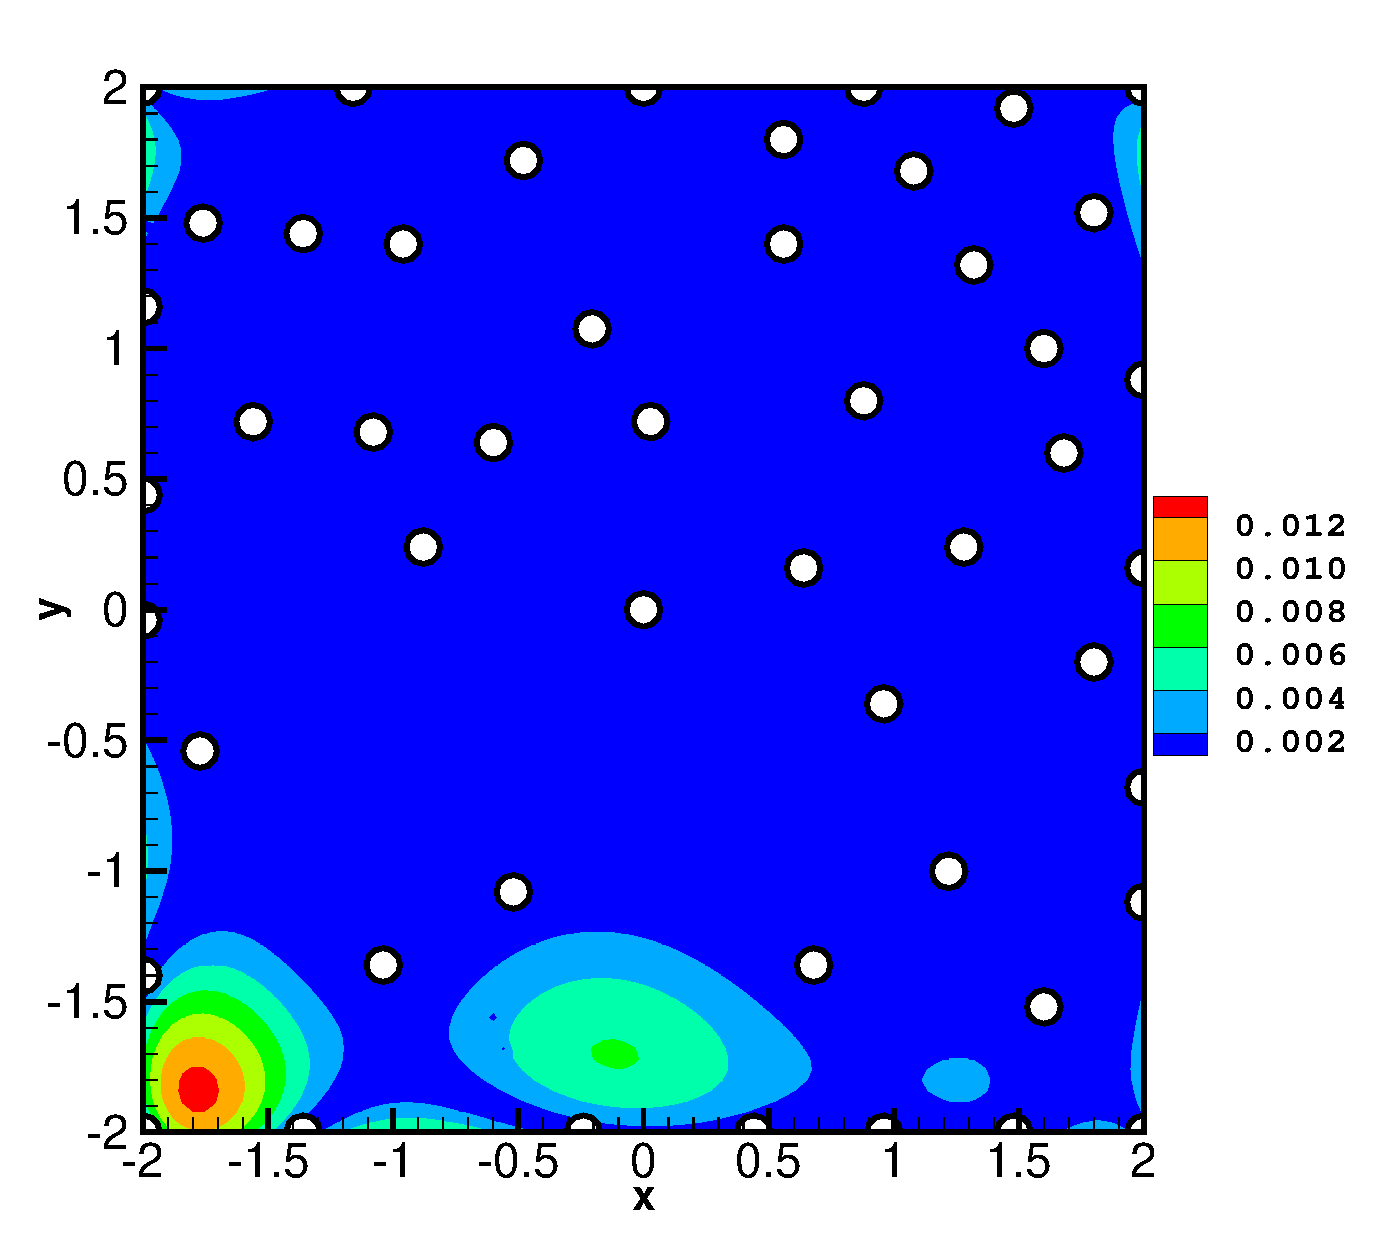
\includegraphics[width=1.0\textwidth]{MIRErrorExp50.eps} %\caption{Cosine}
\end{minipage}
\begin{minipage}[b]{0.32\linewidth}
  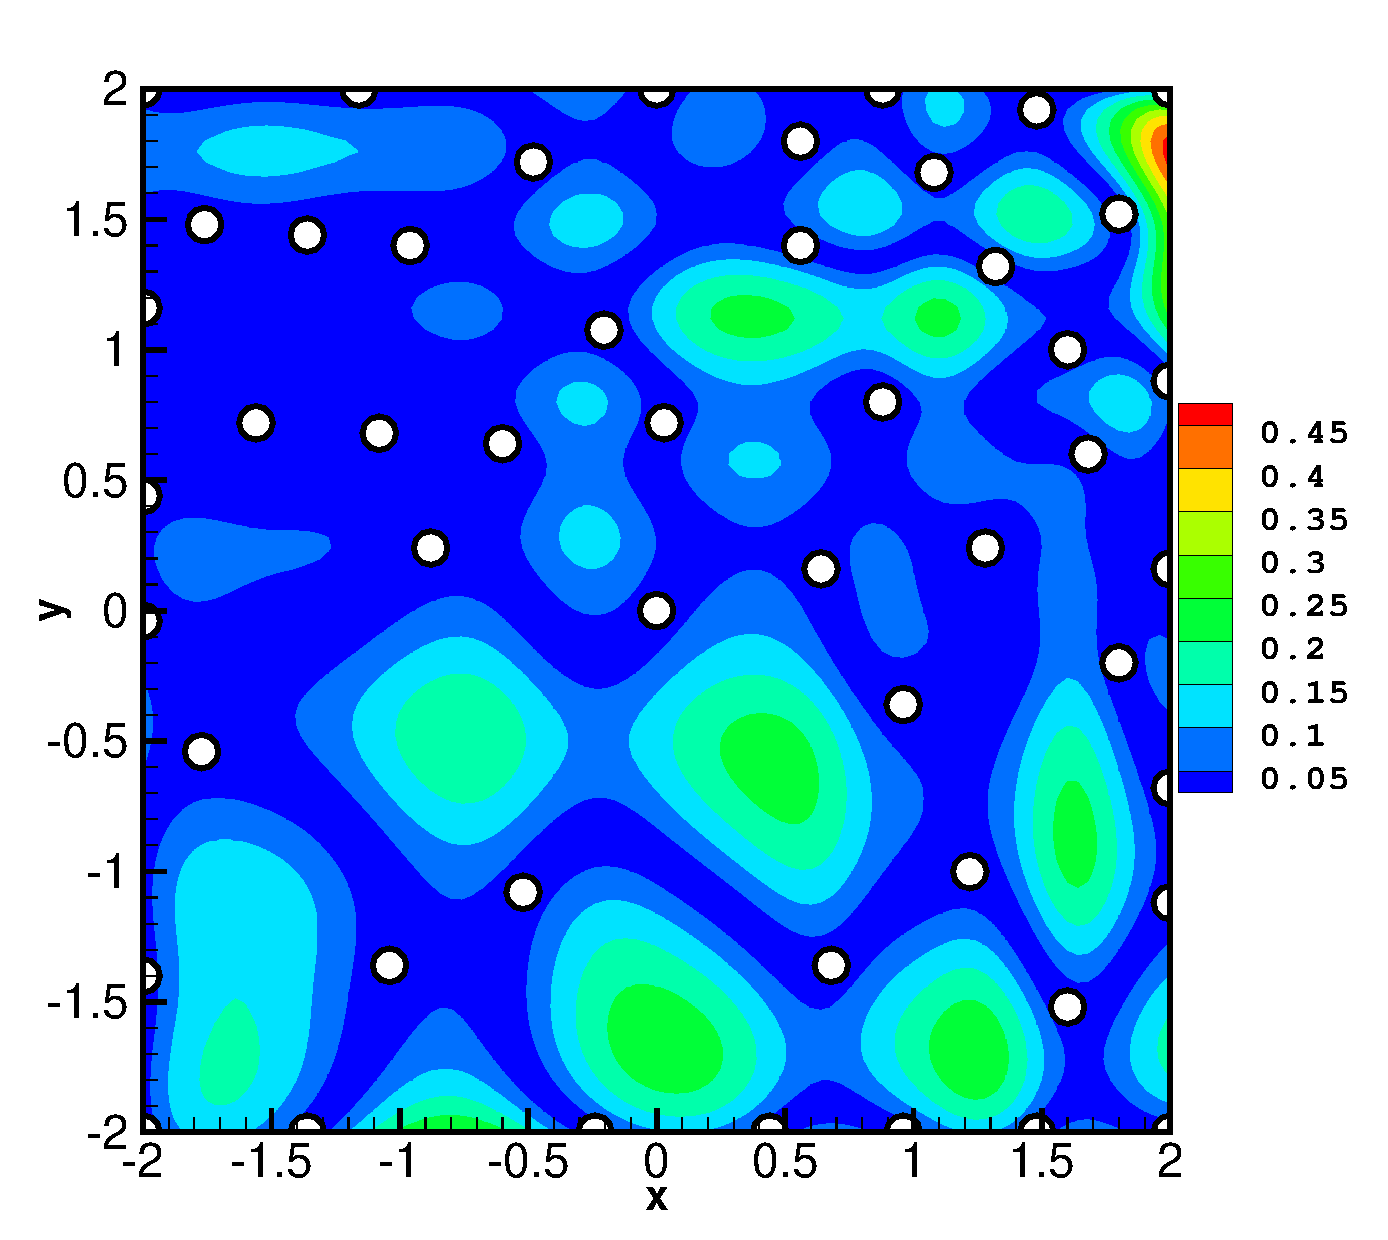
\includegraphics[width=1.0\textwidth]{ErrorExp50.eps} %\caption{Runge}
\end{minipage}
\begin{minipage}[b]{0.32\linewidth}
  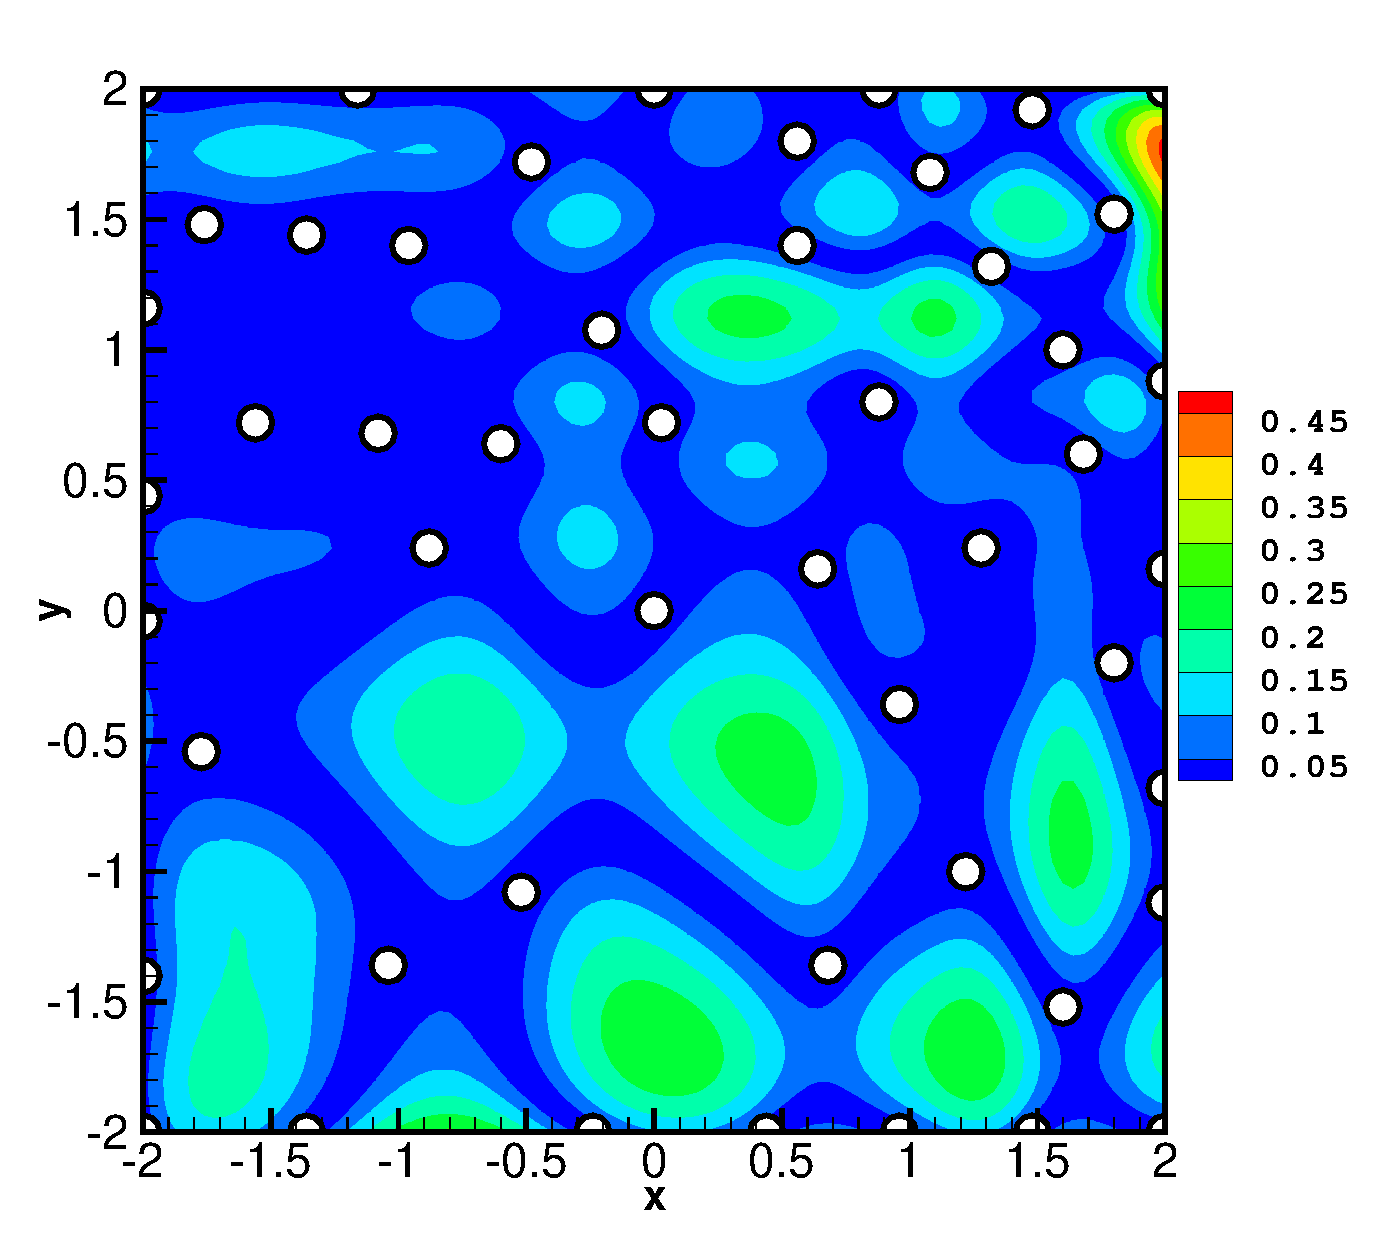
\includegraphics[width=1.0\textwidth]{DiscExp50.eps} %\caption{Exponential}
\end{minipage}
\caption[Error distribution for exponential test function.]{Contour plots for the exponential test function showing the distribution of: the local surrogate model error (left), the global kriging surrogate model error (middle) and the  proposed discrepancy function (right). 
The global and local surrogate models are built with 50 and 25 training points (white circles), respectively.}
\label{Expdist}
\end{figure}
\begin{figure}[h]
  \centering
\begin{minipage}[b]{0.32\linewidth}
  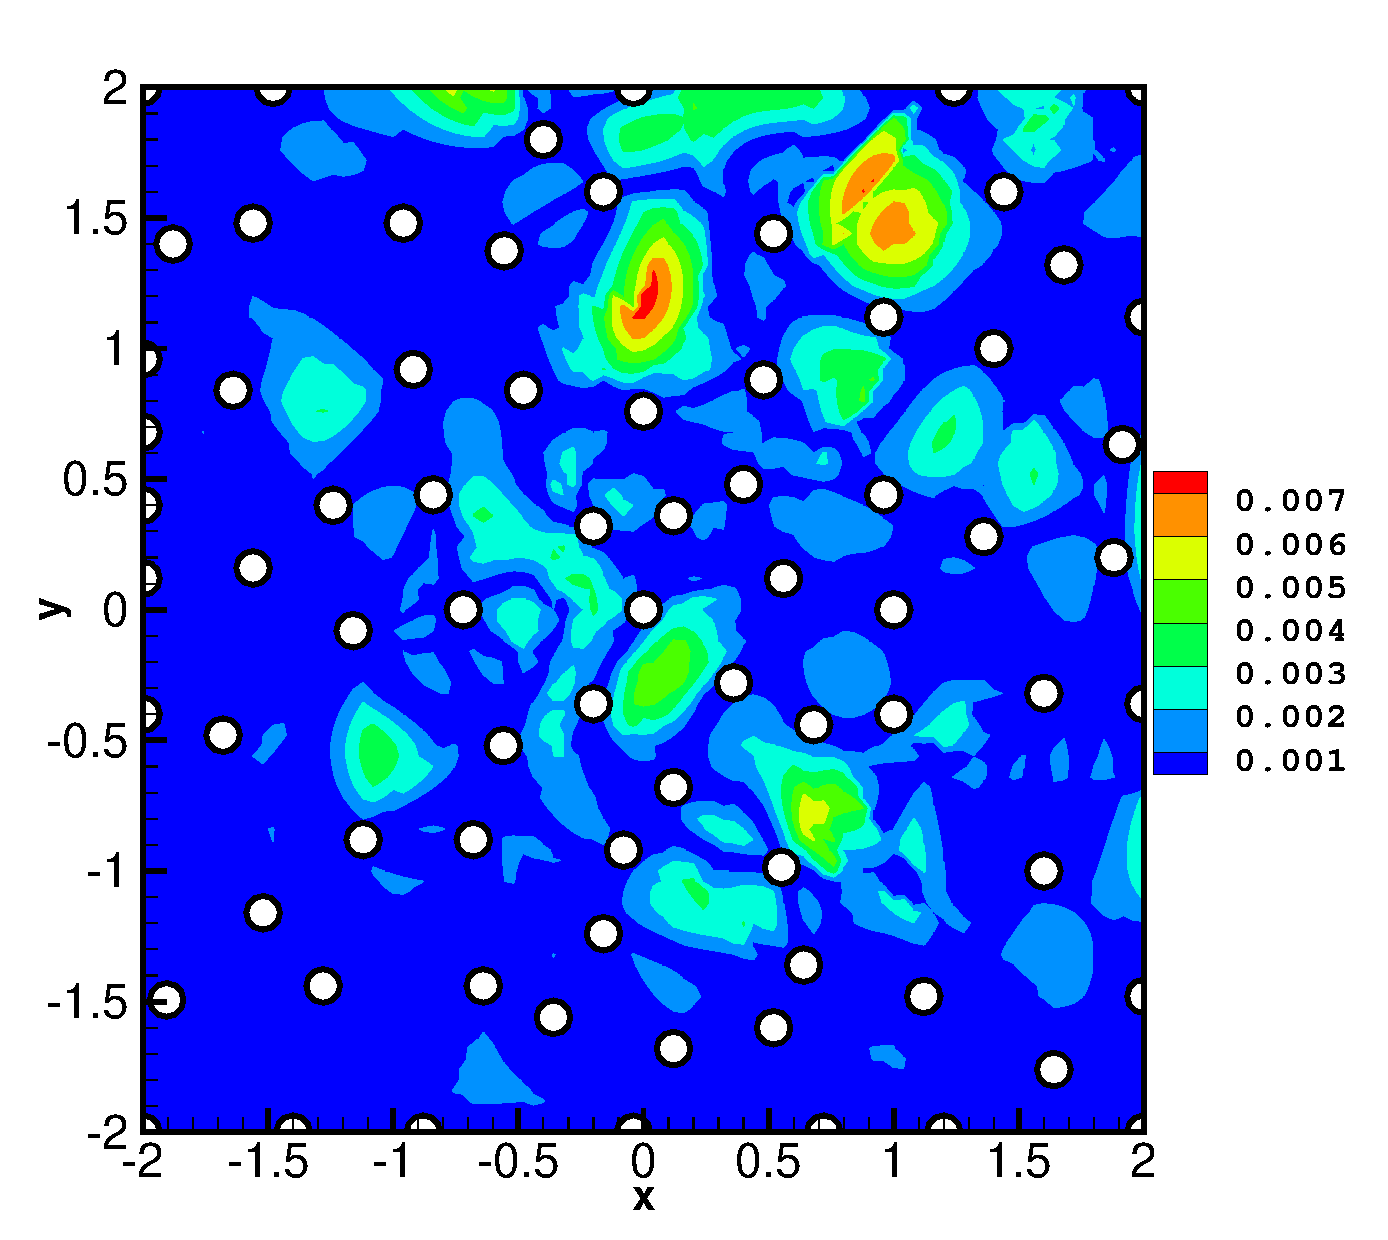
\includegraphics[width=1.0\textwidth]{MIRErrorRunge75.eps} %\caption{Cosine}
\end{minipage}
\begin{minipage}[b]{0.32\linewidth}
  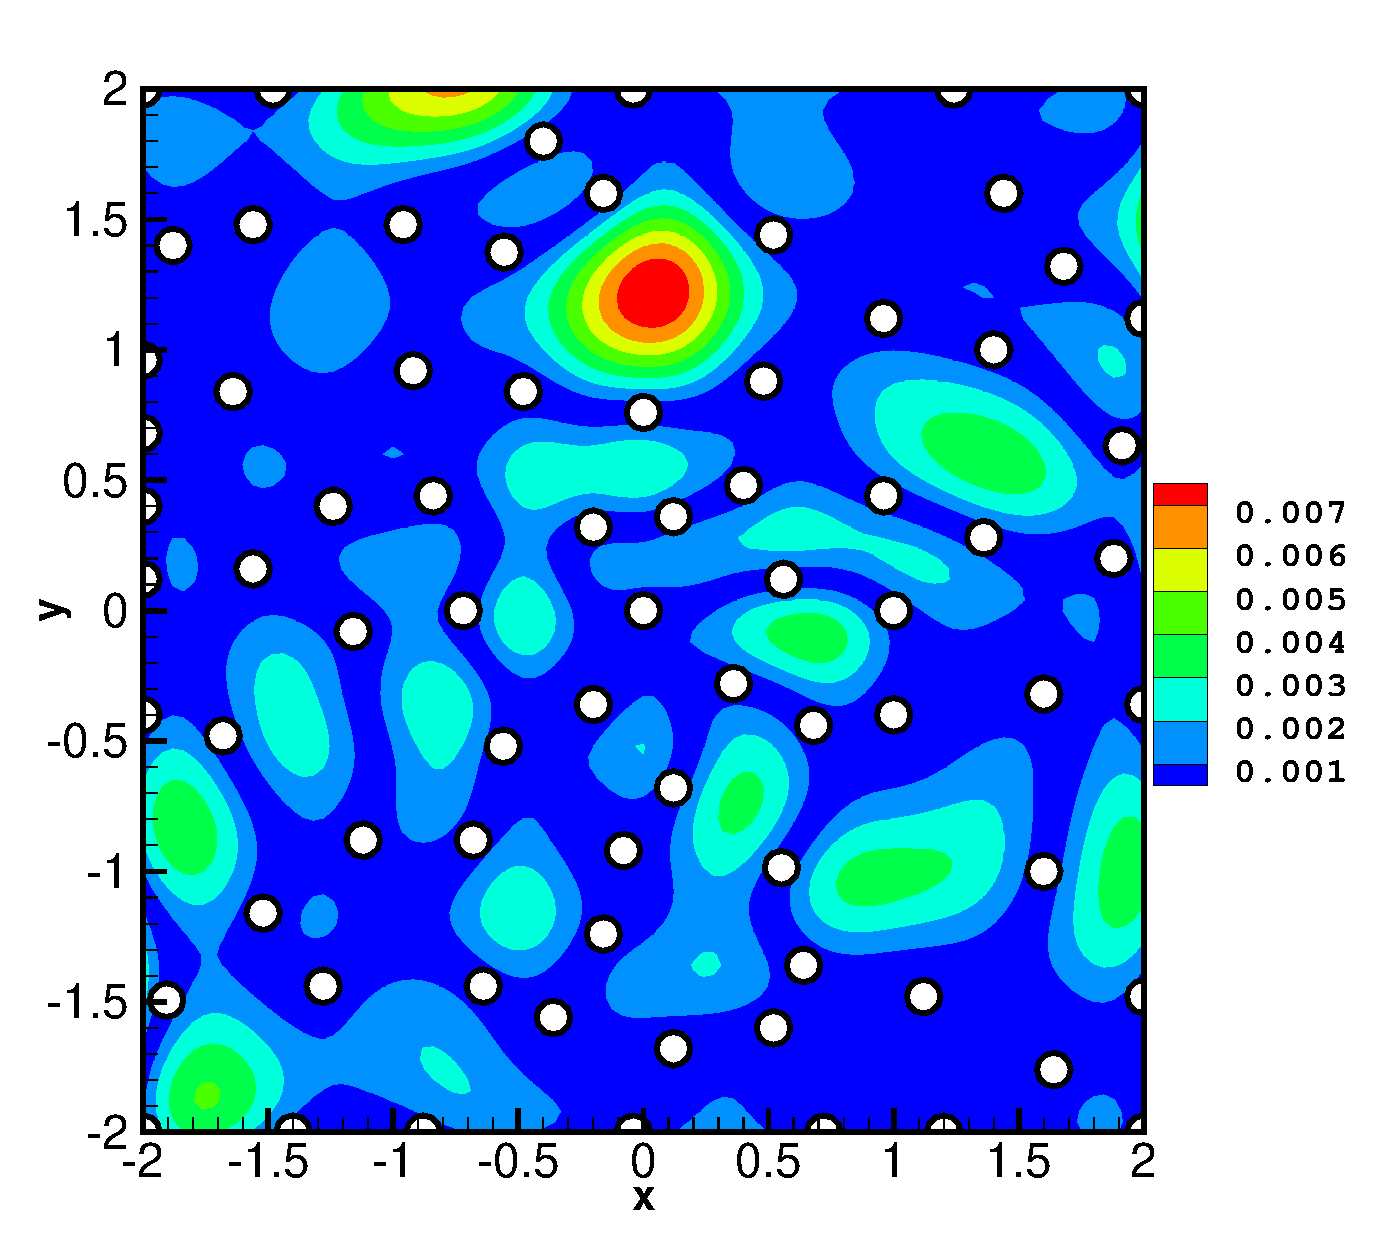
\includegraphics[width=1.0\textwidth]{ErrorRunge75.eps} %\caption{Runge}
\end{minipage}
\begin{minipage}[b]{0.32\linewidth}
  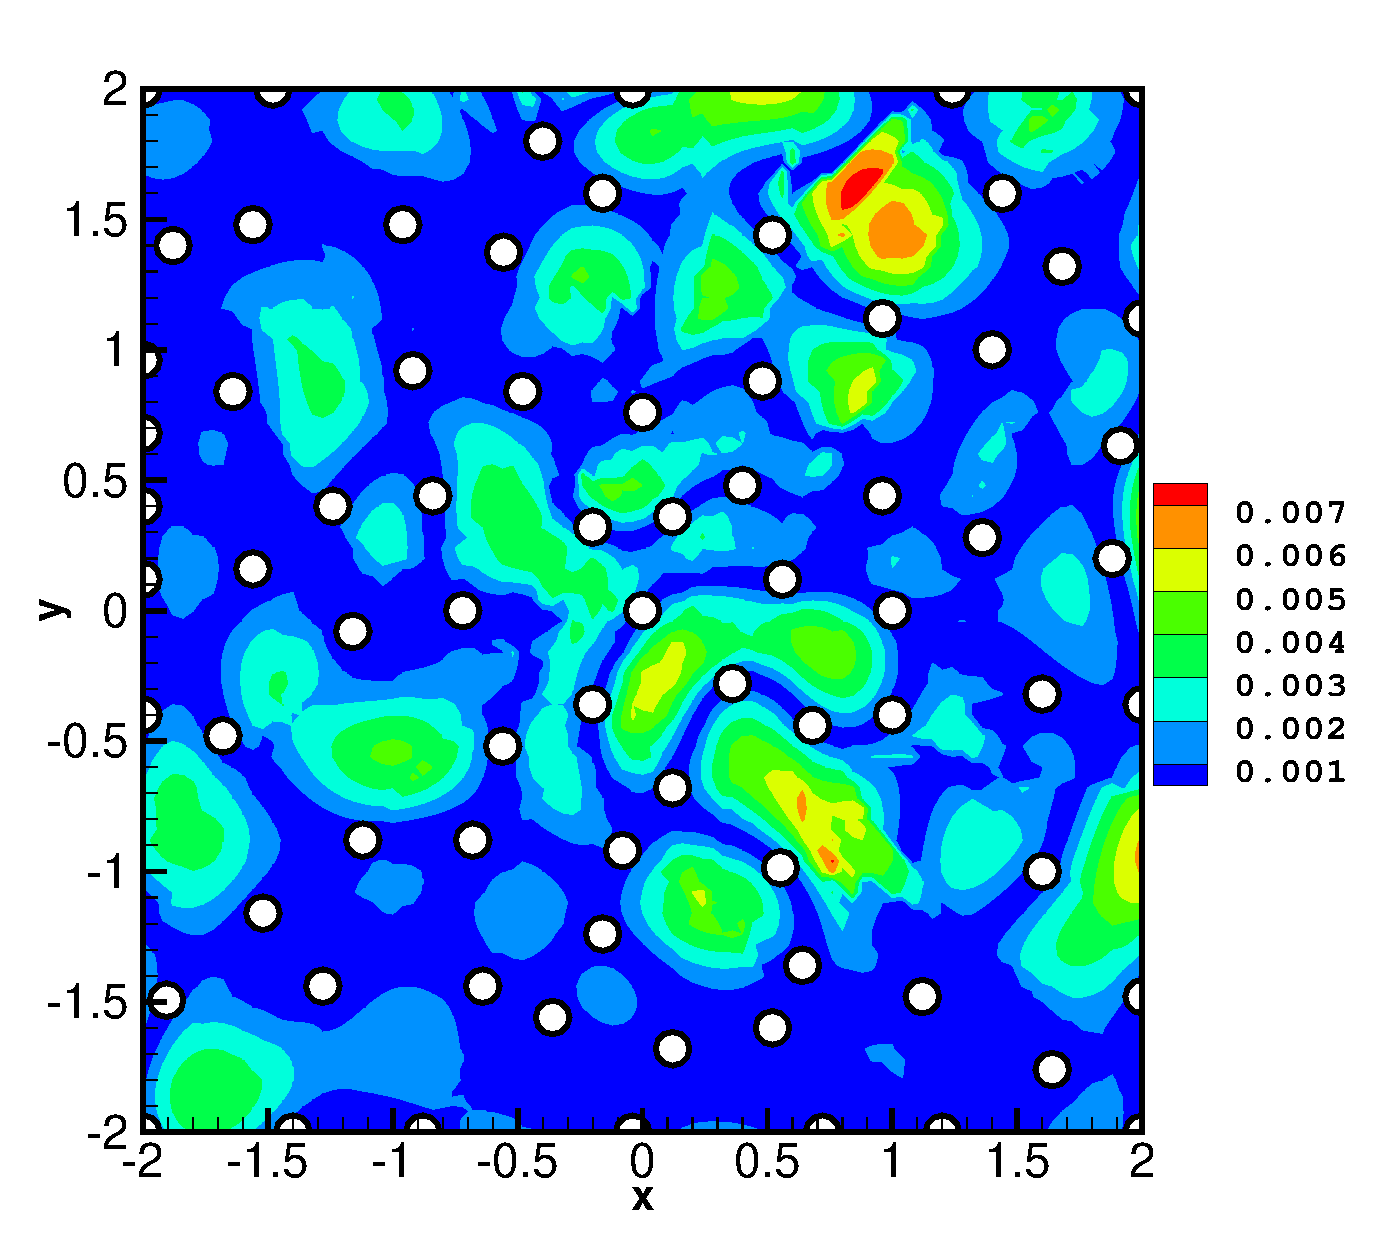
\includegraphics[width=1.0\textwidth]{DiscRunge75.eps} %\caption{Exponential}
\end{minipage}
\caption[Error distribution for Runge test function.]{Contour plots for the Runge test function showing the distribution of: the local surrogate model error (left), the global kriging surrogate model error (middle) and the  proposed discrepancy function (right). 
The global and local surrogate models are built with 75 and 25 training points (white circles), respectively.}
\label{Rungedist}
\end{figure}
\begin{figure}[h]
  \centering
\begin{minipage}[b]{0.32\linewidth}
  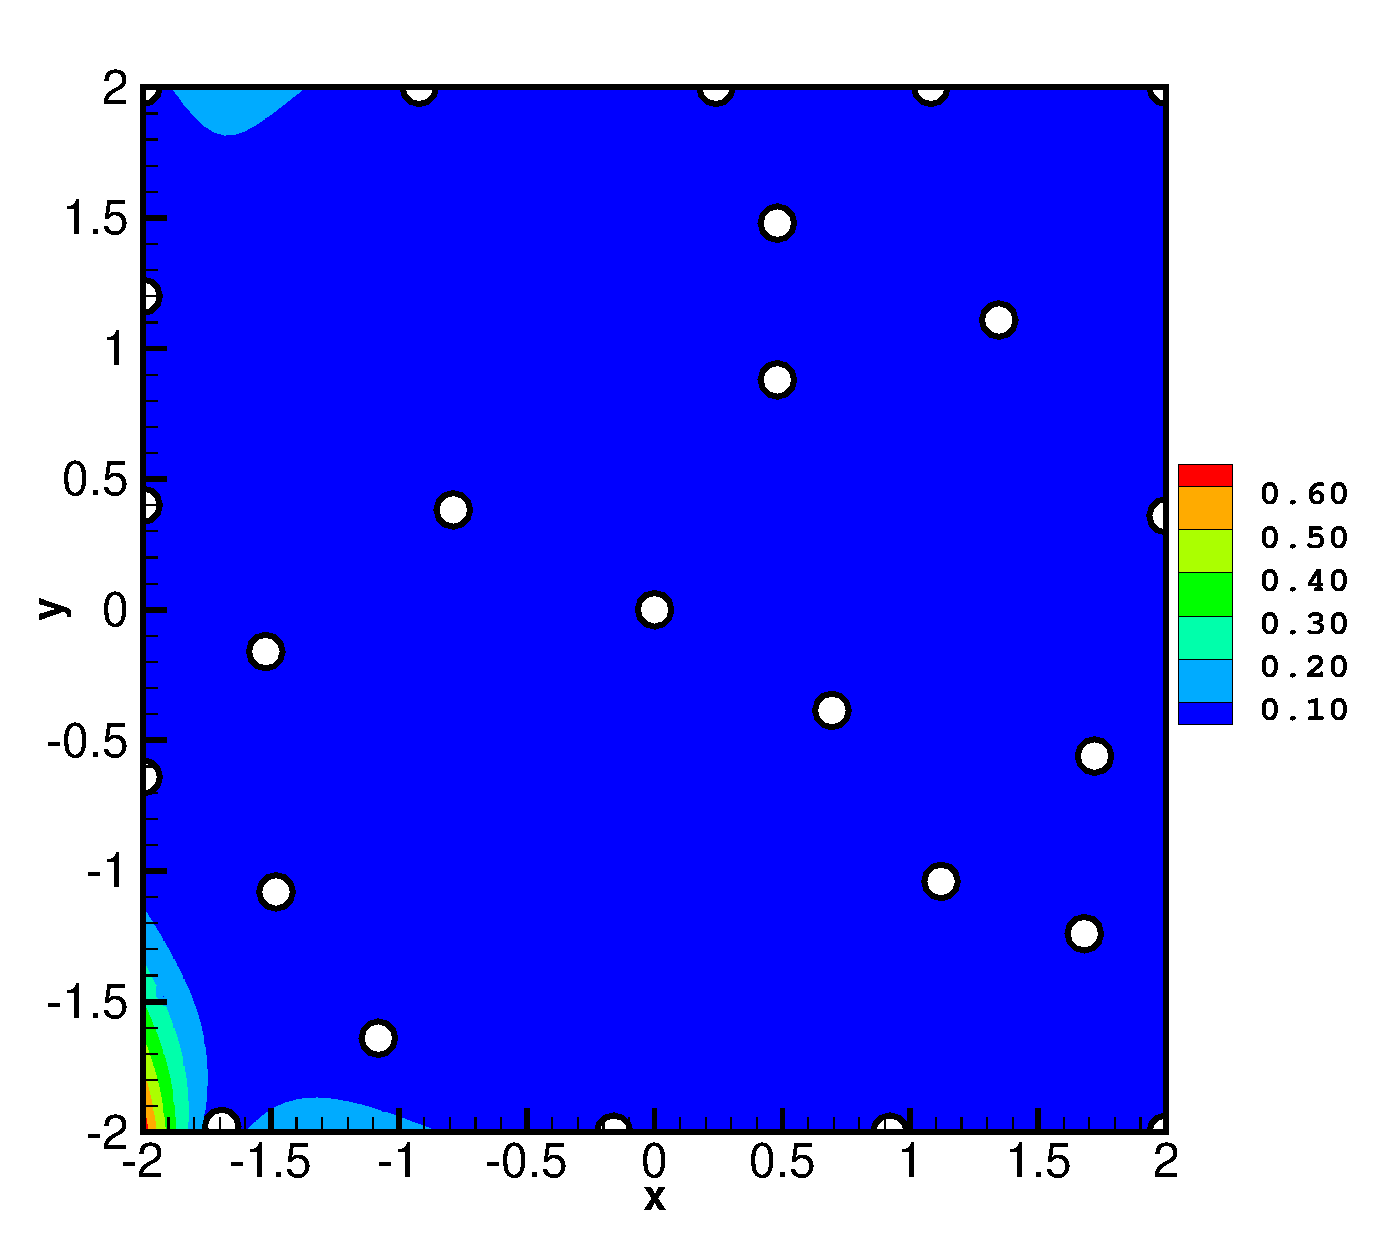
\includegraphics[width=1.0\textwidth]{MIRErrorRosen25.eps} %\caption{Cosine}
\end{minipage}
\begin{minipage}[b]{0.32\linewidth}
  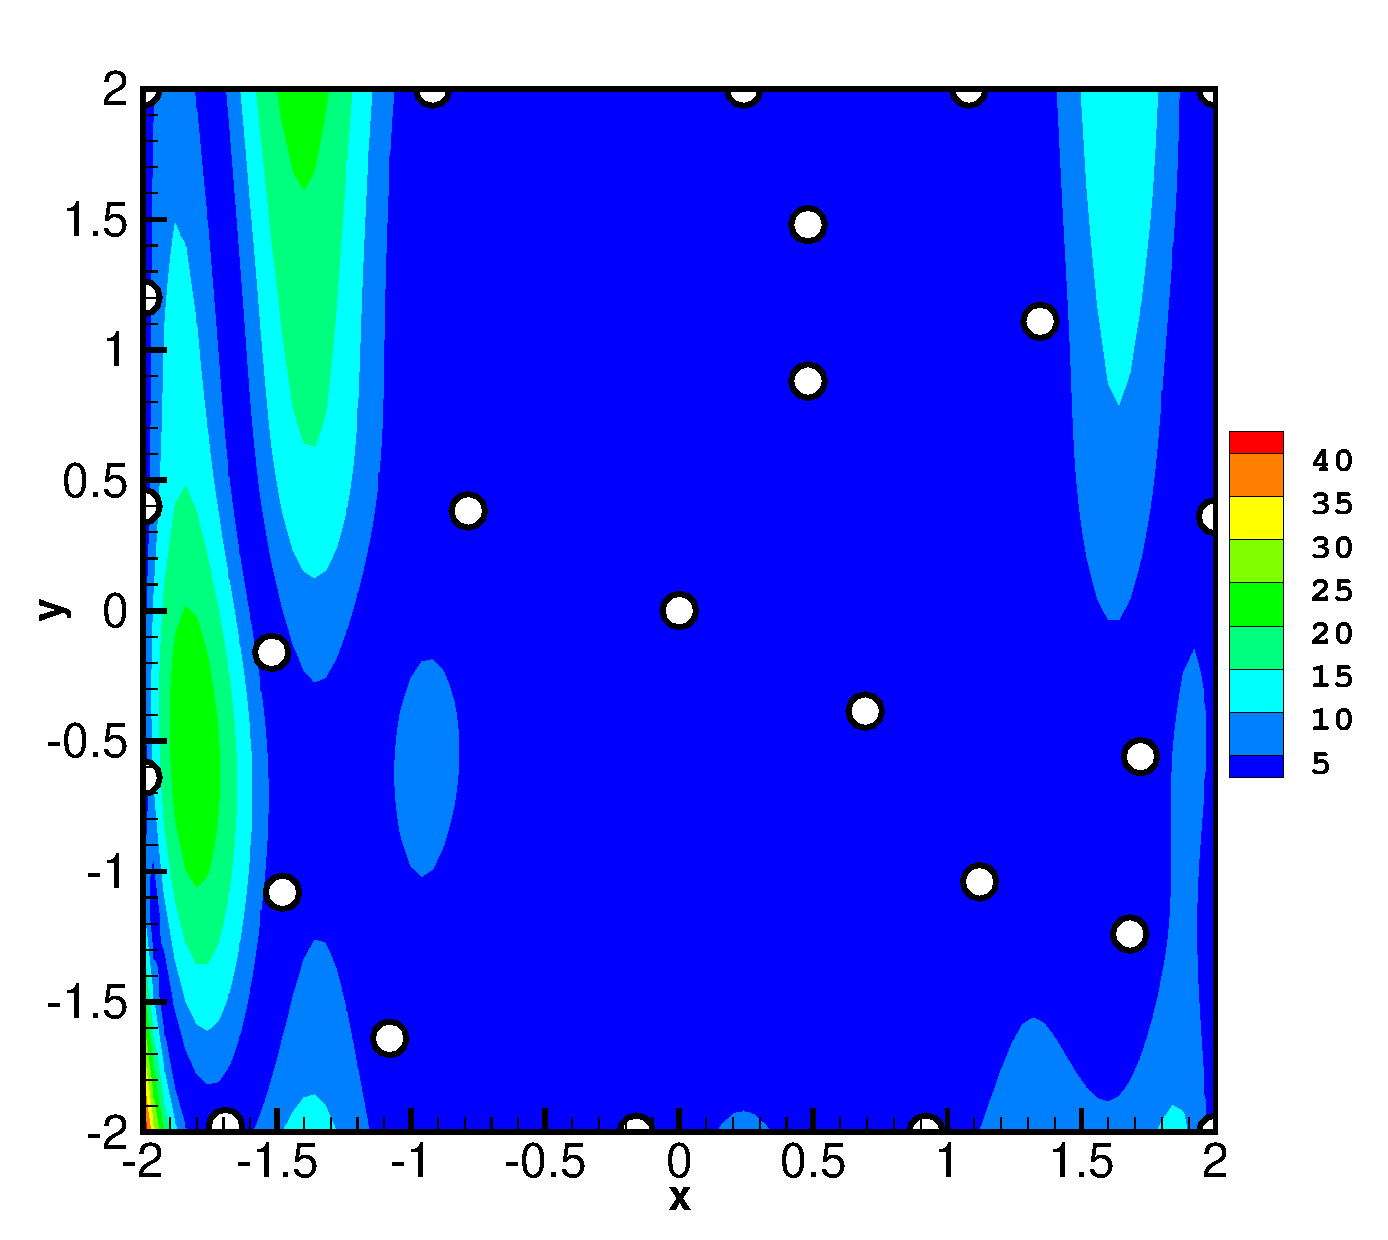
\includegraphics[width=1.0\textwidth]{ErrorRosen25.eps} %\caption{Runge}
\end{minipage}
\begin{minipage}[b]{0.32\linewidth}
  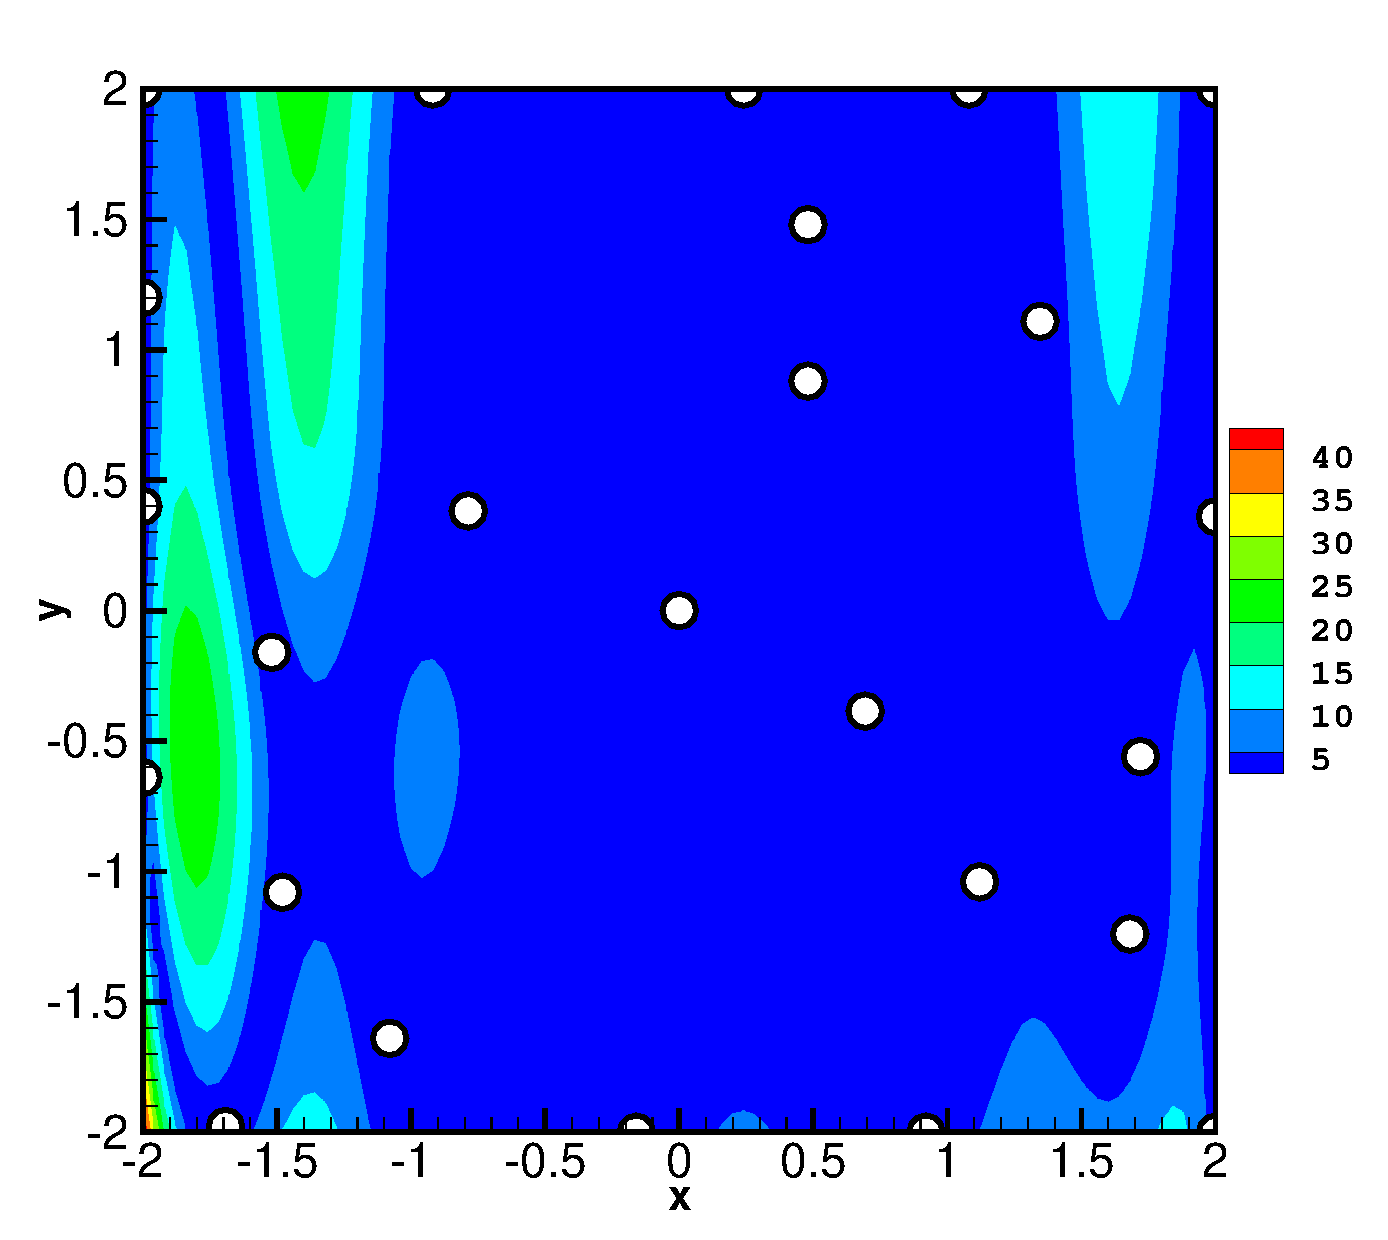
\includegraphics[width=1.0\textwidth]{DiscRosen25.eps} %\caption{Exponential}
\end{minipage}
\caption[Error distribution for Rosenbrock test function.]{Contour plots for the Rosenbrock test function showing the distribution of: the local surrogate model error (left), the global kriging surrogate model error (middle) and the proposed discrepancy function (right). 
The global and local surrogate model(s) are both built with 25 training points (white circles).}
\label{Rosendist}
\end{figure}

%\caption{Contour plots showing the values predicted by the global kriging surrogate model (top left), local MIR surrogate models (top right), the distribution of actual error in the model (bottom left) and the distribution of the proposed discrepancy function (bottom right) using Runge test function. The global and local surrogate models are built with 75 and 25 training points, respectively.}


The differences between the function predictions of the two surrogate models (local and global) is proposed as an approximation to the actual error in the global surrogate model as discussed in section~\ref{dynamic}. From Figures~\ref{Expdist},~\ref{Rungedist} and~\ref{Rosendist} a close agreement can be noticed between the global surrogate model's actual error distribution (middle) and the proposed discrepancy function (right), which explains the excellent trends shown in Figures~\ref{diffrmsekrig} and ~\ref{diffrmsePCE}. 
Only for the Runge function (see Figure~\ref{Rungedist}) can differences be visually seen between the actual error and the proposed discrepancy function.
 Similar plots for PCE are not shown here, but the behavior is clearly evident from the presented trends.


Generally, it is possible for the local surrogate models to provide less accurate representation of the domain, especially when only a few training points are available. 
Therefore, it is advisable to use all the available training data to build local surrogate model(s) during the first few selection cycles. 
For example, in this work the local surrogate models for the two-dimensional cases use all the available training data until the size of the training data set increases beyond 25, after which it is fixed at 25 for computational efficiency purposes. Nevertheless, the accuracy of the local surrogate models is \emph{not a strict requirement}, as they can still be used as reference models to build and validate the global surrogate.


As a final remark, if the training point selection process is desired to be continued, the framework would choose points where the discrepancies shown in the rightmost contour plots of Figures~\ref{Expdist},~\ref{Rungedist} and~\ref{Rosendist} are large (distance-constraint will also be checked before evaluating the expensive exact function).


\section{Kriging Results}

\subsection{Number of Training Points per Cycle}




The proposed dynamic training point selection features a progressive evolution of the training data set for the global surrogate model. 
The user specifies the {number} of training points ($N_{cyc}$) to be added at each iteration to the training data set - a factor that determines the
rate at which the final training data set is evolved.
In the case of PCE, the surrogate is built in steps of one polynomial order per  selection cycle and the required number of additional points can be determined from Eq.~(\ref{numberofterms}) and the chosen oversampling factor which is two. In the case of kriging, the choice of $N_{cyc}$ is left to the user as kriging does not mandate any requirements on the minimum number of points needed to build the surrogate.
It is recommended to add a moderate number of training points per iteration
to facilitate a \textit{better evolution} of the training data set.
Adding only a few points per cycle implies more computational burden since the kriging (also PCE or any response surface) has to be constructed more often to reach a fixed number of training points.


\begin{figure}[h!]
\centering
\begin{minipage}[b]{0.32\linewidth}
  \includegraphics[width=1.0\textwidth]{ncycstudyexp.eps} \subcaption{Exponential}
\end{minipage}
\begin{minipage}[b]{0.32\linewidth}
  \includegraphics[width=1.0\textwidth]{ncycstudyrunge.eps} \subcaption{Runge}
\end{minipage}
\begin{minipage}[b]{0.32\linewidth}
  \includegraphics[width=1.0\textwidth]{ncycstudyrosen.eps} \subcaption{Rosenbrock}
\end{minipage}
\caption[A study on the number of training points selected per cycle.]{The effect of the number of training points selected per cycle on the accuracy  for two-dimensional test functions using kriging.}
\label{ntps}
\end{figure} 


Figure~\ref{ntps} shows the effect of the number of training points added per iteration on the accuracy of the global surrogate for all three analytical test functions in two dimensions.
The training can be done by choosing more points per cycle, to reduce the number of times the surrogate model needs to be built, as the general monotonic behavior is preserved for all the tested cases (two, five and ten) and also because the trade-off with accuracy is found to be small.  For the two-dimensional Rosenbrock test function, the kriging surrogate model does not present a monotone behavior after reaching about 40 training points, due to failed tuning of kriging hyper-parameters. A similar chaotic convergence behavior was observed for other polynomial test functions such as the quadratic and cubic ones (results are not shown here).
It will be shown later (see section~\ref{Comparison with kriging MSE}) that kriging exhibits the same behavior with all the tested training point selection approaches.

\begin{figure}[h!]
\centering
\begin{minipage}[b]{0.32\linewidth}
  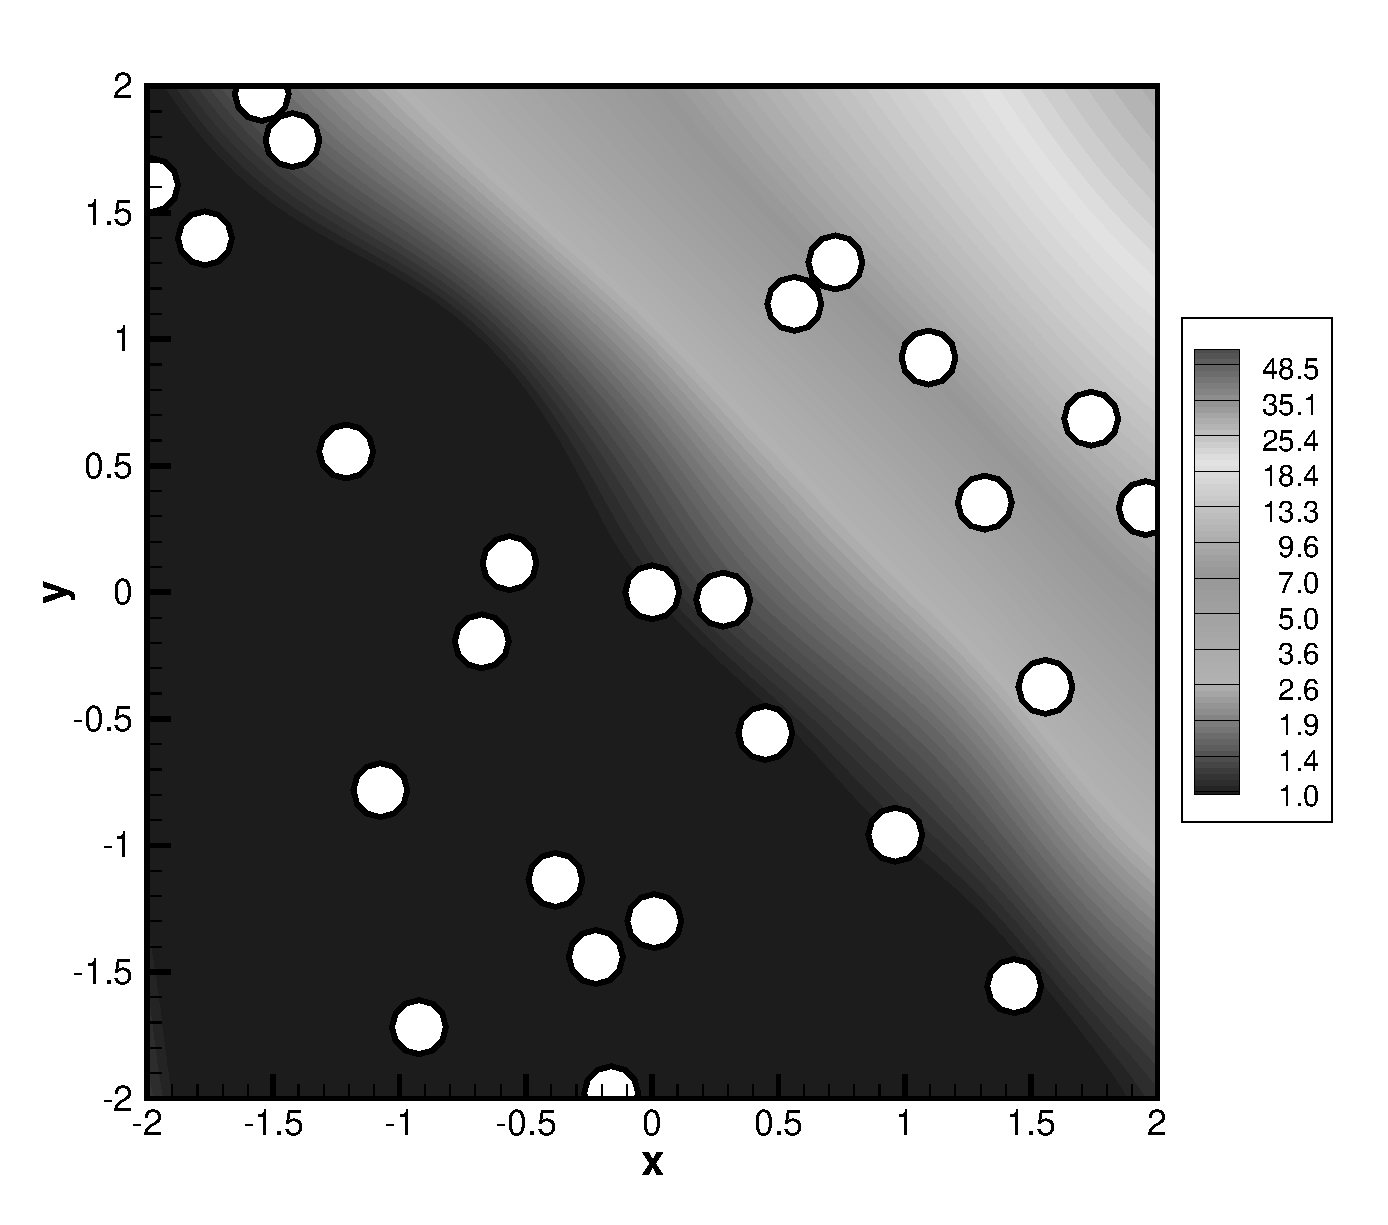
\includegraphics[width=1.0\textwidth]{kriging02dlhs.eps} 
\end{minipage}
\begin{minipage}[b]{0.32\linewidth}
  \includegraphics[width=1.0\textwidth]{kriging22dlhs.eps} 
\end{minipage}
\begin{minipage}[b]{0.30\linewidth}
  \includegraphics[width=1.0\textwidth]{kriging32dlhs.eps} 
\end{minipage}
\begin{minipage}[b]{0.32\linewidth}
  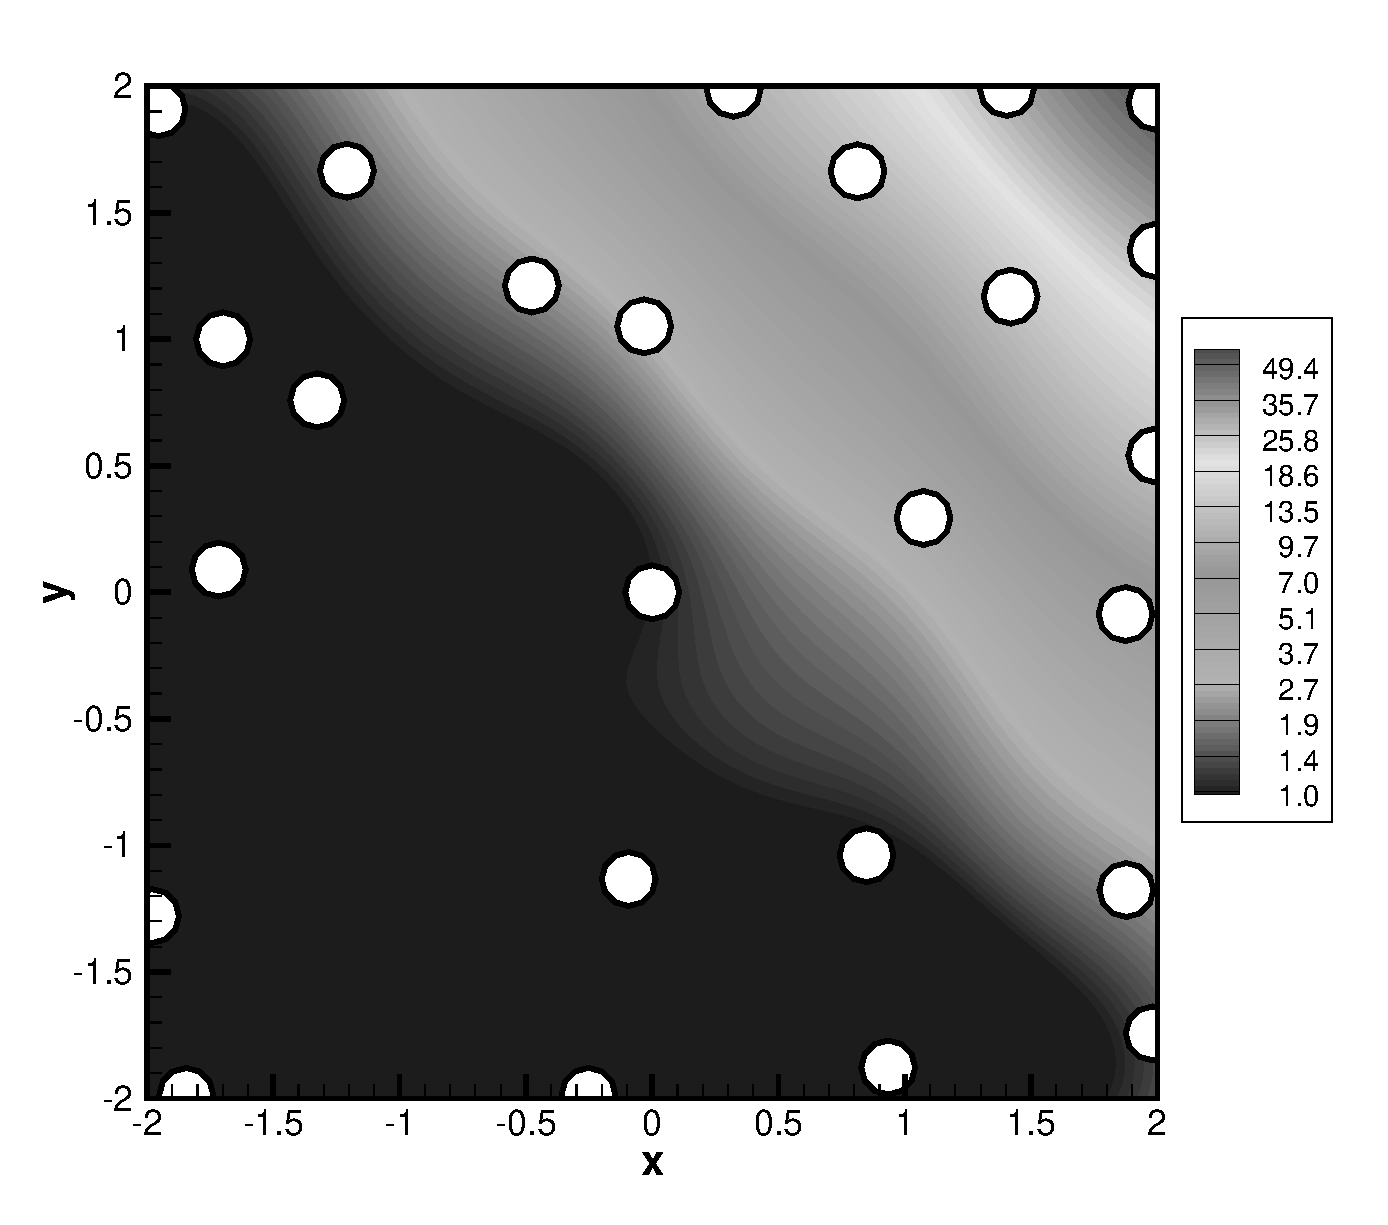
\includegraphics[width=1.0\textwidth]{kriging02ddyn.eps} \subcaption{Exponential}
\end{minipage}
\begin{minipage}[b]{0.32\linewidth}
  \includegraphics[width=1.0\textwidth]{kriging22ddyn.eps} \subcaption{Runge}
\end{minipage}
\begin{minipage}[b]{0.32\linewidth}
  \includegraphics[width=1.0\textwidth]{kriging32ddyn.eps} \subcaption{Rosenbrock}
\end{minipage}
\caption[Training point distributions using the proposed framework.]{Training point distributions ($N=25$) for two-dimensional test functions using LHS (top) and the dynamic method (bottom). }
\label{ltps2d}
\end{figure}
\subsection{Training Point Distribution}


Figure~\ref{ltps2d} shows typical training point distributions for all three test functions using LHS as well as the proposed dynamic method using kriging. 
In this example, five points were selected per iteration until reaching the final training data set with $25$ points.
It can be observed that the dynamic training strategy concentrates training points in regions where the curvature is high, near the
peaks and bounds, and in regions where the points are sparse. 
For example, the top row of Figure~\ref{ltps2d} (corresponding to latin hypercube sampling) has larger unsampled regions in the domain
than the bottom row (dynamic training), where the training points are more spread throughout the domain. 
Such a strategy can save a lot of computational time when applied to high-fidelity simulations by reducing the number of required function
evaluations to produce a globally accurate surrogate model. On the other hand, LHS tends to miss important locations as well as affects the matrix conditioning through too closely spaced points. 


\subsection{Accuracy of Dynamically Enhanced Kriging Surrogate Model}
A quantitative comparison of the accuracy of the dynamically trained (and thereby enhanced) kriging surrogate model will be provided in the following paragraphs by means of RMSE comparisons.
\subsubsection{Comparison with Low-discrepancy Sequences using Kriging}
\begin{figure}[h!]
\centering
\begin{minipage}[b]{0.32\linewidth}
  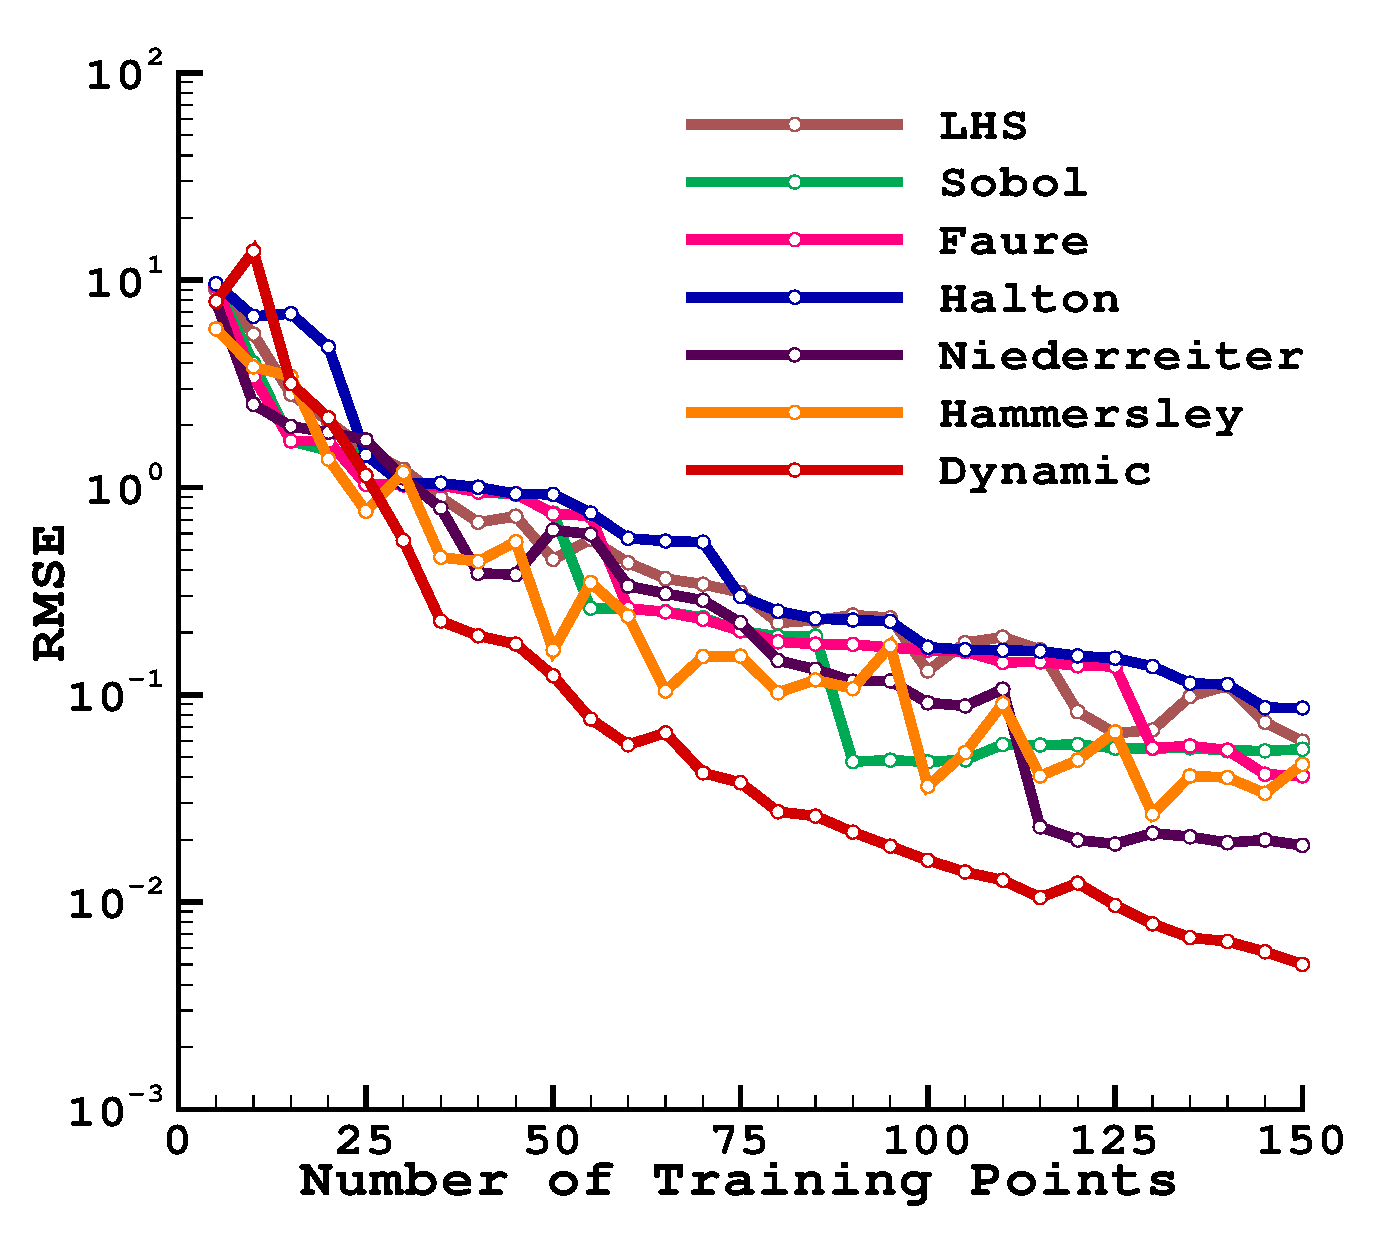
\includegraphics[width=1.0\textwidth]{sequencesfct00.eps}\subcaption{Exponential}
\end{minipage}
\begin{minipage}[b]{0.32\linewidth}
  \includegraphics[width=1.0\textwidth]{sequencesfct02.eps}\subcaption{Runge}
\end{minipage}
\begin{minipage}[b]{0.32\linewidth}
 \includegraphics[width=1.0\textwidth]{sequencesfct03.eps}\subcaption{Rosenbrock}
\end{minipage}
\caption[Dynamic method versus quasi-random sequences.]{A comparison of the dynamic training point selection with some quasi-Monte Carlo sequences and LHS on two-dimensional test functions using kriging.}
\label{quasimc}
\end{figure} 
The dynamic training point selection is compared with some quasi-Monte Carlo sequences such as Sobol, Faure, and Halton. LHS is also included in the comparisons to show its performance compared to other strategies.
From  Figure~\ref{quasimc}, it can be seen that the dynamic training point selection is better at producing accurate surrogate models than the other approaches. As discussed above, for the Rosenbrock test function all training point selection strategies suffer from chaotic convergence with kriging due to the choice of spatial correlation function.

\subsubsection{Comparison with Kriging MSE Minimization}
\label{Comparison with kriging MSE}
The kriging surrogate model provides an error estimate through the expected mean squared error (MSE) as described earlier. The MSE can be used to guide the training point selection process by adding training points at locations where the MSE is large. 
Figure~\ref{krigingmse} shows a comparison of kriging surrogate models built with LHS, minimizing MSE and the proposed framework for training point selection.
For all three test functions, the proposed framework produces more accurate surrogate models. 

\begin{figure}[h!]
\centering
\begin{minipage}[b]{0.32\linewidth}
  \includegraphics[width=1.0\textwidth]{msefct00.eps}\subcaption{Exponential}
\end{minipage}
\begin{minipage}[b]{0.32\linewidth}
  \includegraphics[width=1.0\textwidth]{msefct02.eps}\subcaption{Runge}
\end{minipage}
\begin{minipage}[b]{0.32\linewidth}
 \includegraphics[width=1.0\textwidth]{msefct03.eps}\subcaption{Rosenbrock}
\end{minipage}
\caption[Dynamic method versus MSE minimization method.]{A comparison of the dynamic training point selection with minimizing the MSE method on two-dimensional test functions using kriging. LHS is also included to show its relative performance.}
\label{krigingmse}
\end{figure} 


For the Rosenbrock function $f_3$, the MSE method features a poor convergence after about 40 training points and is even outperformed by LHS. 
In order to alleviate the non-smooth convergence behavior of kriging for the Rosenbrock test function (using LHS, Sobol, Faure, Halton, MSE, and the proposed framework) other spatial correlation functions 
have been employed and the results are displayed in Figure~\ref{krigingscf}. 
\begin{figure}[h!]
\centering
\begin{minipage}[b]{0.32\linewidth}
  \includegraphics[width=1.0\textwidth]{gaussian03.eps}
\end{minipage}
\begin{minipage}[b]{0.32\linewidth}
  \includegraphics[width=1.0\textwidth]{spline03.eps}
\end{minipage}
\caption[Comparing spatial correlation functions of kriging.]{A comparison of accuracies of the kriging model built with Gaussian (left) and spline (right) spatial correlation functions for two-dimensional Rosenbrock test function.}
\label{krigingscf}
\end{figure} 
By comparing the rightmost Figure~\ref{krigingmse} (using Wendland C4) with Figure~\ref{krigingscf} (using Gaussian and spline) it can be noted that spline spatial correlation functions feature a much smoother convergence when compared to Wendland C4 and Gaussian spatial correlation functions. 
However, since a derivative-enhanced kriging model is employed in this work, Wendland C4 spatial correlation function~\cite{Wendland2005} is used as default for the remainder of this article to ensure differentiability.
%The developed dynamic training point selection produces more accurate surrogate models compared to other DoE techniques on all these spatial correlation functions and all DoE methods tested.
%as it is widely used within the surrogate modeling community as well as
Also, for further comparisons only LHS will be considered to reduce the complexity in presenting the results. 


\subsection{Dynamic versus LHS in 2D}
 
In order to account for the inherent randomness in LHS all two-dimensional results are averaged over ten separate runs and the mean results are presented with bounds 
referring to the best and worst case.

\begin{figure}[h!]
\centering
\begin{minipage}[b]{0.32\linewidth}
  \includegraphics[width=1.0\textwidth]{KRIerrorbarFct00dim02F.eps} \subcaption{Exponential}
\end{minipage}
\begin{minipage}[b]{0.32\linewidth}
  \includegraphics[width=1.0\textwidth]{KRIerrorbarFct02dim02F.eps}\subcaption{Runge}
\end{minipage}
\begin{minipage}[b]{0.32\linewidth}
  \includegraphics[width=1.0\textwidth]{KRIerrorbarFct03dim02F.eps}\subcaption{Rosenbrock}
\end{minipage}
\caption[Dynamic method versus LHS using kriging in 2D (F only).]{Plots comparing training point selections using LHS and the dynamic method on two-dimensional test functions (with function values only) with kriging. Five training points are selected per cycle.}
\label{krigingRMSin2D}
\end{figure}
\begin{figure}[h!]
\centering
\begin{minipage}[b]{0.32\linewidth}
  \includegraphics[width=1.0\textwidth]{KRIerrorbarFct00dim02GH.eps}\subcaption{Exponential}
\end{minipage}
\begin{minipage}[b]{0.32\linewidth}
  \includegraphics[width=1.0\textwidth]{KRIerrorbarFct02dim02GH.eps}\subcaption{Runge}
\end{minipage}
\begin{minipage}[b]{0.32\linewidth}
  \includegraphics[width=1.0\textwidth]{KRIerrorbarFct03dim02GH.eps}\subcaption{Rosenbrock}
\end{minipage}
\caption[Dynamic method versus LHS using kriging in 2D (FG and FGH).]{Plots comparing training point selections using LHS and the dynamic method on two-dimensional test functions (with derivative information) with kriging. Five training points are selected per cycle.}
\label{krigingRMSin2DD}
\end{figure}

From Figure~\ref{krigingRMSin2D} it can be inferred that the dynamic method
(shown with continuous lines) performs better than LHS (shown with dashed lines), both in terms of monotonicity and accuracy.
The dynamic training point selection improves the accuracy of the surrogate by roughly an order of magnitude when compared to LHS, 
for the first two test functions. For the Rosenbrock test function ($f_3$), though not as distinct as for the other test functions, 
the lower bounds show that the dynamic method is still more accurate than LHS.


The training point selection in the presence of derivative information is shown separately in Figure~\ref{krigingRMSin2DD}.
It can be noted that the addition of gradient and Hessian information helps to improve the accuracy of the response surface for both LHS and the dynamic training point selection. 
The dynamic training point selection improves the accuracy even more by placing the higher-order derivative information in the most viable locations.
This behavior can be observed across all test functions in Figure~\ref{krigingRMSin2DD}. Also, it can be seen that the LHS Hessian cases (FGH) of $f_1$ and $f_3$ (Figure~\ref{krigingRMSin2DD} left and right, respectively), are not more accurate than the gradient cases (FG) as expected. But with the dynamic method, auxiliary information always improves the accuracy of the surrogate model, as it ably chooses the locations that would contain derivative information.


The smaller bounds on the RMSE for the dynamic method in the figures indicate that it is less random than LHS implying that only one run is sufficient whereas most random training point selection methods require multiple runs to ensure
that ``bad luck'' does not impede the results. 
In most instances, the upper bounds of the dynamic method (corresponding to its worst approximation) are still better than the lower bounds of LHS (corresponding to its best approximation). 
Hence it can be expected that the dynamic training point selection method to produce more accurate surrogates for a fixed computational budget. 
The superiority of the dynamic method over other quasi-Monte Carlo sequences has already been demonstrated in Figure~\ref{quasimc}.

\subsection{Dynamic versus LHS in 5D}
\begin{figure}[h!]
\centering
\begin{minipage}[b]{0.32\linewidth}
  \includegraphics[width=1.0\textwidth]{rmsekrgdim5fct0.eps} \subcaption{Exponential}
\end{minipage}
\begin{minipage}[b]{0.32\linewidth}
  \includegraphics[width=1.0\textwidth]{rmsekrgdim5fct2.eps}\subcaption{Runge}
\end{minipage}
\begin{minipage}[b]{0.32\linewidth}
  \includegraphics[width=1.0\textwidth]{rmsekrgdim5fct3.eps}\subcaption{Rosenbrock}
\end{minipage}
\caption[Dynamic method versus LHS using kriging in 5D.]{Plots comparing training point selections using LHS and the dynamic method on five-dimensional test functions with kriging. Fifty training points are selected per cycle.}
\label{krigingRMSin5D}
\end{figure} 

Figure~\ref{krigingRMSin5D} shows the results for five-dimensional test functions. Due to the computational resources needed to build five-dimensional surrogate models, error bounds are not included. 
It can be seen that the dynamic method (shown as continuous lines) helps to improve the accuracy of the kriging surrogate compared to LHS (shown as dashed lines).
The advantage of including derivative information is also more evident for these higher-dimensional test cases. 

As a general remark, if the proposed dynamic training point selection (or any response-based method) is used, the surrogate is built progressively starting from an initial (small) number of training points, to achieve better accuracy for a fixed computational budget. 
The cost of building the surrogate model multiple times can generally be neglected in comparison with the computational cost of high-fidelity physics-based simulations. 
If the surrogate construction should become too expensive, it can be accelerated by selecting a larger number of additional training points per cycle for a minimal trade-off with accuracy as demonstrated in Figure~\ref{ntps}.





\section{Polynomial Chaos Results}\label{pcresults}

Results pertaining to the polynomial chaos expansions are discussed in this section. An oversampling factor of two is enforced to improve the matrix conditioning (prevents accidental rank deficiency).
The dynamic training point selection is initiated by building a second-order accurate PCE including a training point at the center of the domain. As the order of expansion increases, the required number of collocation points (training points) are picked dynamically. 

\subsection{Dynamic versus LHS in 2D}

Figure~\ref{rms2dpceF} compares PCE with LHS (shown as dashed lines) with that of PCE with dynamic training point selection (shown as continuous lines) for all three test functions, along with error bounds similar to the results presented for kriging.
As it can be seen, the convergence behavior of PCE with LHS is chaotic compared to that of the dynamic strategy which is monotonic instead. 
Although the rational Runge function ($f_2$) is known to pose difficulties for PCE~\cite{Constantine2013}, the dynamic method shows good convergence whereas LHS shows very poor results.
Note that recently a rational polynomial chaos expansion scheme has been developed by Sheshadri~\etal~\cite{Constantine2013} to address the difficulty of PCE with such functions.
The fourth-order polynomial Rosenbrock function ($f_3$) is captured exactly after the order of expansion reaches four; however, it suffers from polynomial over-fitting (using a model that is more sophisticated than needed)~\cite{overfitting} as the order of expansion increases further.
Overall, the dynamic training point selection consistently produces more accurate surrogates compared to LHS.
Figure~\ref{rms2dpceGH} shows the improved performance of the dynamic method for choosing training points that contain gradient (labeled FG) and Hessian information (labeled FGH). 
In particular, for the Runge function, the advantage of the proposed framework is very pronounced.  



\begin{figure}[h!]
\centering
\begin{minipage}[b]{0.32\linewidth}
  \includegraphics[width=1.0\textwidth]{PCErrorbarFct04dim02F.eps} \subcaption{Exponential}
\end{minipage}
\begin{minipage}[b]{0.32\linewidth}
  \includegraphics[width=1.0\textwidth]{PCErrorbarFct02dim02F.eps} \subcaption{Runge} 
\end{minipage}
\begin{minipage}[b]{0.32\linewidth}
  \includegraphics[width=1.0\textwidth]{PCErrorbarFct06dim02F.eps}  \subcaption{Rosenbrock}
\end{minipage}
\caption[Dynamic method versus LHS using PCE in 2D (F only).]{Plots comparing training point selections using LHS and the dynamic method on two-dimensional test functions (function values only) with PCE. The order of expansion, $p$, ranges from 2 to 11.}
\label{rms2dpceF}
\end{figure}
\begin{figure}[h!]
\centering
\begin{minipage}[b]{0.32\linewidth}
  \includegraphics[width=1.0\textwidth]{PCErrorbarFct04dim02GH.eps}  \subcaption{Exponential}
\end{minipage}
\begin{minipage}[b]{0.32\linewidth}
  \includegraphics[width=1.0\textwidth]{PCErrorbarFct02dim02GH.eps}  \subcaption{Runge}
\end{minipage}
\begin{minipage}[b]{0.32\linewidth}
  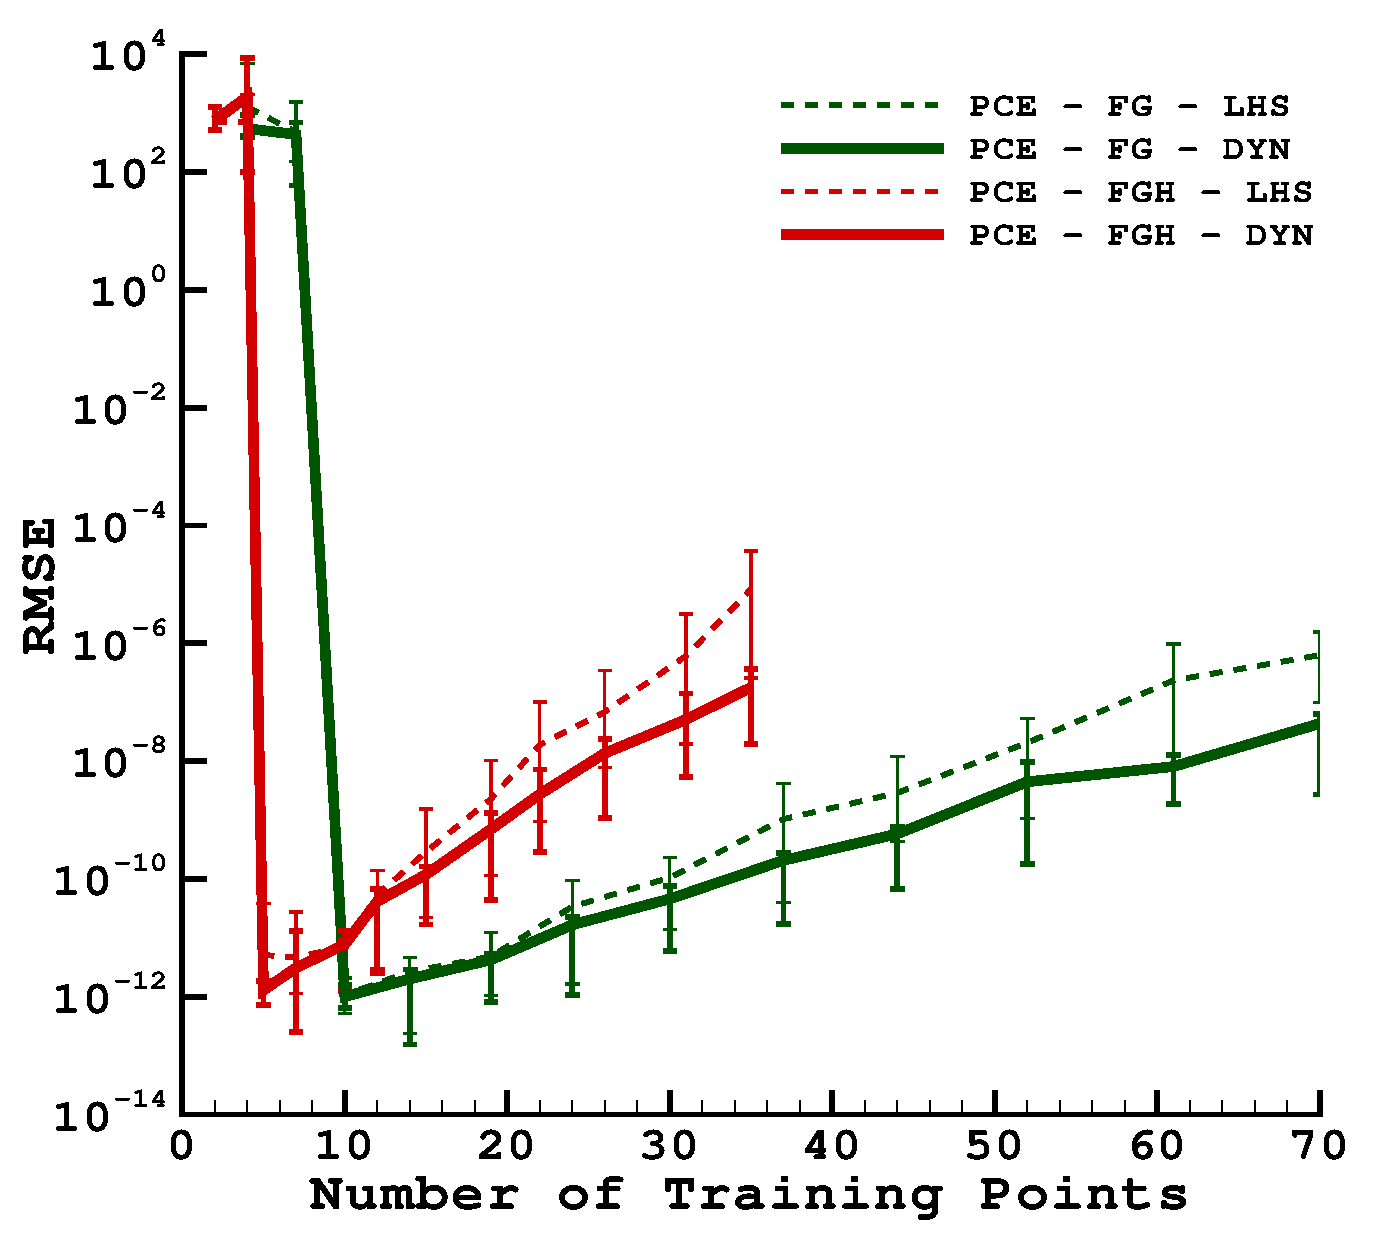
\includegraphics[width=1.0\textwidth]{PCErrorbarFct06dim02GH.eps}  \subcaption{Rosenbrock}
\end{minipage}
\caption[Dynamic method versus LHS using PCE in 2D (FG and FGH).]{Plots comparing training point selections using LHS and the dynamic method on two-dimensional test functions (with higher-order derivative information) with PCE. The order of expansion, $p$, ranges from 2 to 12.}
\label{rms2dpceGH}
\end{figure}

\subsection{Dynamic versus LHS in 5D}

Figure~\ref{rmse5dpc} the shows five-dimensional results.
It is again evident that the dynamic method is more consistent in producing a good PCE surrogate compared to LHS which tends to show random fluctuations.
% It is to be noted that the importance of derivative information is more evident in this higher dimensional test case. 
When the function values alone are used, about $6000$ training points are needed for a tenth order polynomial. If gradients are used, only about $1000$ points are needed and only about $200$ points are required with function, gradient and Hessian information to roughly obtain the same level of accuracy. This is because of the availability of additional training information as discussed in section~\ref{curseofdimensionality}.


\begin{figure}[h!]
\centering
\begin{minipage}[b]{0.32\linewidth}
  \includegraphics[width=1.0\textwidth]{rmsepcdim5fct4.eps}  \subcaption{Exponential}
\end{minipage}
\begin{minipage}[b]{0.32\linewidth}
  \includegraphics[width=1.0\textwidth]{rmsepcdim5fct2.eps} \subcaption{Runge}
\end{minipage}
\begin{minipage}[b]{0.32\linewidth}
  \includegraphics[width=1.0\textwidth]{rmsepcdim5fct6.eps}  \subcaption{Exponential}
\end{minipage}
\caption[Dynamic method versus LHS using PCE in 5D.]{Plots comparing training point selections using LHS and the dynamic method on five-dimensional test functions. The order of expansion, $p$, ranges from 2 to 10.}
\label{rmse5dpc}
\end{figure} 

\subsection{Validation of Gradients and Hessian from Surrogate}
Figures~\ref{approxgradhess} and \ref{approxgradhess5d} show the RMSE between the approximated
function (shown as blue lines), gradients (shown as green lines) and
Hessian (shown as red lines) with that of the exact values in two and five dimensions, respectively.
It can be seen that the PCE produces good approximations of gradient and Hessian information that can be used for many applications including optimization and uncertainty quantification.
\begin{figure}[h!]
\centering
\begin{minipage}[b]{0.32\linewidth}
  \includegraphics[width=1.0\textwidth]{rmsepcgraddim2fct4.eps}  \subcaption{Exponential} 
\end{minipage}
\begin{minipage}[b]{0.32\linewidth}
  \includegraphics[width=1.0\textwidth]{rmsepcgraddim2fct2.eps} \subcaption{Runge}
\end{minipage}
\begin{minipage}[b]{0.32\linewidth}
  \includegraphics[width=1.0\textwidth]{rmsepcgraddim2fct6.eps} \subcaption{Rosenbrock}
\end{minipage}
\caption[Approximated derivatives from PCE in 2D.]{RMSE in the approximated function, gradient and Hessian values from PCE for two-dimensional test functions.}
\label{approxgradhess}
\end{figure} 
\begin{figure}[h!]
\centering
\begin{minipage}[b]{0.32\linewidth}
  \includegraphics[width=1.0\textwidth]{rmsepcgraddim5fct4.eps} \subcaption{Exponential}
\end{minipage}
\begin{minipage}[b]{0.32\linewidth}
  \includegraphics[width=1.0\textwidth]{rmsepcgraddim5fct2.eps} \subcaption{Runge}
\end{minipage}
\begin{minipage}[b]{0.32\linewidth}
  \includegraphics[width=1.0\textwidth]{rmsepcgraddim5fct6.eps} \subcaption{Rosenbrock}
\end{minipage}
\caption[Approximated derivatives from PCE in 5D.]{RMSE in the approximated function, gradient and Hessian values from PCE for five-dimensional test functions.}
\label{approxgradhess5d}
\end{figure} 

\subsection{Choice of Orthogonal Polynomials}
All the results shown above for PCE use Legendre orthogonal
basis. Results in Figure~\ref{polystudy} show the effect of using
different orthogonal polynomials to construct the basis matrix
$\psi$. For a reasonable comparison, the same set of training points (chosen via LHS) that were
used with  Legendre orthogonal basis were also used with Hermite orthogonal basis. 
Though the PCE coefficients $\bm{u}$ are found to be different when using Hermite polynomials as basis, it did not show any impact on the overall accuracy of the PCE surrogate model, as polynomial interpolation is unique. For $f_3$ small
deviations can be seen only after reaching machine precision (not due to the choice of basis). % A similar behavior was observed for the five-dimensional test cases as well (results are not shown here).
\begin{figure}[h!]
\centering
\begin{minipage}[b]{0.32\linewidth}
  \includegraphics[width=1.0\textwidth]{legherexp.eps} \subcaption{Exponential}
\end{minipage}
\begin{minipage}[b]{0.32\linewidth}
  \includegraphics[width=1.0\textwidth]{legherrun.eps} \subcaption{Runge}
\end{minipage}
\begin{minipage}[b]{0.32\linewidth}
  \includegraphics[width=1.0\textwidth]{legherrosen.eps} \subcaption{Rosenbrock}
\end{minipage}
\caption[Choice of basis function for PCE.]{A comparison between Legendre and Hermite basis functions for PCE in two dimensions.}
\label{polystudy}
\end{figure} 

\section{Comparison of Kriging and Polynomial Chaos}
The purpose of this section is to compare the kriging and PCE surrogates, both of which are enhanced with the dynamic training point selection method on analytical test functions.
%\subsection{Two-dimensional test cases}
\begin{figure}[h!]
\centering
\begin{minipage}[b]{0.32\linewidth}
\includegraphics[width=1.0\textwidth]{rmse2dkpcexp.eps} \subcaption{Exponential}
\end{minipage}
\begin{minipage}[b]{0.32\linewidth}
\includegraphics[width=1.0\textwidth]{rmse2dkpcrun.eps} \subcaption{Runge}
\end{minipage}
\begin{minipage}[b]{0.32\linewidth}
\includegraphics[width=1.0\textwidth]{rmse2dkpcrosen.eps}  \subcaption{Rosenbrock}
\end{minipage}
\caption[Kriging versus PCE in 2D.]{A comparison between kriging and PCE on two-dimensional test functions.}
\label{kvm2d}
\end{figure}
In Figure~\ref{kvm2d} for the exponential function $f_1$, PCE exhibits a smoother as well as
better convergence rate for all the three subcases F, FG and FGH, than
kriging. Whereas for the rational Runge function $f_2$, the kriging is producing a better
surrogate than PCE. The Rosenbrock function $f_3$ is captured exactly
by PCE as expected, whereas kriging is converging much slower (as it is not a polynomial based surrogate). For all the kriging test cases five training points were added per cycle.
%\subsection{Five-dimensional test cases}
Figure~\ref{kvm5d} compares kriging with PCE for the five-dimensional test cases.
For $f_1$, PCE performs slightly better than kriging. However, for
$f_2$, PCE produces poor results and $f_3$ is captured exactly as
expected.  In building the kriging surrogate $600$, $100$, and $20$ training points
were selected per cycle for $F$, $FG$, and $FGH$ test cases, respectively.
\begin{figure}[h!]
\centering
\begin{minipage}[b]{0.32\linewidth}
\includegraphics[width=1.0\textwidth]{rmse5dkpcexp.eps} \subcaption{Exponential}
\end{minipage}
\begin{minipage}[b]{0.32\linewidth}
\includegraphics[width=1.0\textwidth]{rmse5dkpcrun.eps} \subcaption{Runge}
\end{minipage}
\begin{minipage}[b]{0.32\linewidth}
\includegraphics[width=1.0\textwidth]{rmse5dkpcrosen.eps}  \subcaption{Rosenbrock}
\end{minipage}
\caption[Kriging versus PCE in 5D.]{A comparison between kriging and PCE on five-dimensional test functions.}
\label{kvm5d}
\end{figure}


\subsection{On using Higher-order Derivative Information}
The following discussion is aimed at providing guidelines for choosing an appropriate combination of training point selection method and incorporation of higher-order derivative information.
Generally, the use of derivative information provides improved surrogate models for both kriging and polynomial chaos, irrespective of whether the training points are chosen dynamically or at random (occasionally LHS shows a deviant behavior).
As discussed in section~\ref{introduction}, efficient gradient and Hessian calculation methods are available for high-fidelity
physics-based simulations and they provide the means to reduce the effects of the ``curse of dimensionality''.


\begin{figure}[h]
\centering
\begin{minipage}[b]{0.32\linewidth}
   \includegraphics[width=1.0\textwidth]{rmse2dkpcexpeqfn.eps}  \subcaption{Exponential}
\end{minipage}
\begin{minipage}[b]{0.32\linewidth}
  \includegraphics[width=1.0\textwidth]{rmse2dkpcruneqfn.eps}  \subcaption{Runge}
\end{minipage}
\begin{minipage}[b]{0.32\linewidth}
  \includegraphics[width=1.0\textwidth]{rmse2dkpcroseneqfn.eps}  \subcaption{Rosenbrock}
\end{minipage}
\caption[Plots with equivalent function evaluations in 2D.]{RMSE versus the number of equivalent function evaluations for two-dimensional test functions using kriging and PCE with dynamic training point selection. 
Reference LHS results with function values only are shown with dashed and continuous gray lines corresponding to kriging and PCE, respectively.}
\label{eqfncomp2d}
\end{figure}
\begin{figure}[h]
\centering
\begin{minipage}[b]{0.32\linewidth}
   \includegraphics[width=1.0\textwidth]{rmse5dkpcexpeqfn.eps}  \subcaption{Exponential}
\end{minipage}
\begin{minipage}[b]{0.32\linewidth}
  \includegraphics[width=1.0\textwidth]{rmse5dkpcruneqfn.eps}  \subcaption{Runge}
\end{minipage}
\begin{minipage}[b]{0.32\linewidth}
  \includegraphics[width=1.0\textwidth]{rmse5dkpcroseneqfn.eps}  \subcaption{Rosenbrock}
\end{minipage}
\caption[Plots with equivalent function evaluations in 5D.]{RMSE versus the number of equivalent function evaluations for five-dimensional test functions using kriging and PCE with dynamic training point selection. 
Reference LHS results with function values only are shown with dashed and continuous gray lines corresponding to kriging and PCE, respectively.}
\label{eqfncomp5d}
\end{figure}


Figures~\ref{eqfncomp2d} and ~\ref{eqfncomp5d} take into account the computational time for calculating the gradient and Hessian, and plot the model accuracy versus the number of equivalent exact function evaluations 
for two- and five-dimensional test functions, respectively. 
For example, the computational time for evaluating $N$ data points with function values only (F), is the same as evaluating $\frac{N}{2}$ points with function and gradient values (FG), which in turn is
the same as $\frac{N}{M+2}$ points with function, gradient and Hessian
information (FGH), using the adjoint method as discussed in section~\ref{curseofdimensionality}, where $M$ is the number of dimensions. From these figures it can be inferred that the gradient enhanced surrogates (FG) are computationally more efficient than the
others (F or FGH). The Hessian enhancement does not yield convincing results as expected; however, it can be expected that the Hessian information in specific locations (such as where data points are sparsely distributed) can be advantageous than to add Hessian information to all training points as done here.

In summary, LHS and some low-discrepancy sequences have been shown to produce less accurate results than the proposed dynamic method. 
Additionally, the computational advantage of building gradient enhanced surrogate models is shown in Figures~\ref{eqfncomp2d} and ~\ref{eqfncomp5d}. 
Hence, based on these observations, the dynamic training point selection in conjunction with the use of gradient information for the construction of surrogate models 
offers the best value.


\subsection{Key Observations for Kriging and PCE}


The following discussion summarizes the performances of kriging and PCE in terms of accuracy, robustness and computational time.
\paragraph{\bf{Accuracy:}} A definite conclusion could not be made on this aspect, as these surrogate models (kriging and PCE) perform differently  for different classes of test functions. PCE features higher convergence rates for smooth and
continuously differentiable functions (e.g., $f_1$) and polynomials
(e.g., $f_3$). However, kriging is well suited for non-smooth, non-polynomial functions ($f_2$). A similar comparison for an aerodynamic test case featuring discontinuities will be  shown in chapter~\ref{Database}.
\paragraph{\bf{Robustness:}} The general applicability of both kriging and PCE are compared below.
\begin{itemize}
\item PCE mandates a specific number of points for a particular order of expansion (due to its mathematical setup). It can be disadvantageous when working with a fixed computational budget or already existing data (e.g. experimental data).

\item As the order of expansion increases for PCE, ``wiggles'' tend to appear in
  the PCE surrogate which is a typical behavior of higher-order
  polynomials which can affect the overall accuracy of the
  surrogate. The kriging surrogate model does not suffer from this
  major drawback as it is  not a polynomial.
\item PCE basis matrix is known to suffer from ill-conditioning (more pronounced in the regression approach). Though an oversampling factor of two or more is suggested, it does not guarantee the well-posedness of the problem.
\item PCE produces good results for smooth and polynomial functions, but most physics-based simulations are neither smooth nor polynomials.
\item Kriging supports the usage of both high- and low-fidelity training points~\cite{Han2012,Han2012b,Han2009,Han2010,Yamazaki2013,Yamazaki2012,Yamazaki2011b} whereas PCE does not have this advantage yet.
\end{itemize}

\paragraph{Computational Time:} PCE is cheaper to build and evaluate than kriging. This is due to comparatively intensive mathematical operations required for the construction of kriging as discussed in section~\ref{kriging}. 
On the other hand, for PCE the most time-intensive operation is finding the inverse of the basis matrix $\bm{\psi}$ for a given set of training data.

%A comparison of kriging and polynomial chaos on an aerodynamic test problem will be shown next in chapter~\ref{Database}.
